\chapter{Variational Autoencoders}\label{chap:vae}
Variational autoencoding neural networks, first introduced by Kingma and Welling in the year 2013, see \cite{kingma2013auto}, differently to ordinary autoencoding neural networks that we already mentioned to be discriminative models, are so called generative models, see \cite[Chapter~5]{cinelli2021variational}. This means that instead of trying to estimate the conditional distribution of $y|x$, where $y$ is a predicted label to an observation $x$, variational autoencoders attempt to capture the entire probability distribution of $Y$. This is very interesting for multiple reasons, since this means that we can simulate and anticipate the evolution of the model output. Hence, we could generate new data based on the captured probability distribution. This will be our ultimate goal in this chapter, considering applications at last.

\section{Probabilistic foundations}\label{sec:prob_foundations}

Before diving into the depths of variational autoencoders, we want to begin by laying the essential probabilistic foundations. As already mentioned, in contrast to ordinary autoencoding neural networks which we discussed in Chapter~\ref{chap:ae} variational autoencoding neural networks attempt to capture the entire probability distribution of $Y$. Therefore, we somehow have to construct a probability distribution and at the same time, take the observed data into consideration. In order to so so, we introduce the concept of conditional probabilities. This we do in the following definition.

\begin{definition}\label{def:cond_prob}
Let $(X,\A)$ and $(Y,\B)$ be measurable spaces and let $\prob$ be a probability measure on $(X\times Y, \A\otimes \B)$. Then we call the map $\prob(\wc|\wc):\B\times X \to [0, 1]$ a \textbf{regular conditional probability} of $\prob$ given $X$, if the following three conditions are satisfied:
\begin{itemize}
\item[(i)]   For all $x\in X$ the map $\prob(\wc|x): \B \to [0,1]$ is a probability measure.
\item[(ii)]  For all $B\in\B$ the map $\prob(B|\wc): X \to [0,1]$ is $\A$-measurable.
\item[(iii)] For all $A\in\A$ and $B\in\B$ we have \begin{align*}
\prob(A\times B) = \int_{X} \mathbb{1}_{A}(x) \prob(B|x)d\prob_X(x),
\end{align*}
where $\prob_X$ is the marginal distribution of $\prob$ on $X$.
\end{itemize}
\end{definition}

In Definition \ref{def:cond_prob} we did not assume the existence of a probability density function. However upon doing so, the regular conditional probability can be quickly computed. Let $\m \otimes \n$ be a $\s$-finite measure on $\A \otimes \B$ such that the probability measure $\prob$ on $\A \otimes \B$ has a $\m \otimes \n$ density $p: X \times Y \to  [0, \infty]$. We define $p_X: X \to [0, \infty]$ by
\begin{align*}
p_X(x) \coloneqq \int_{Y} p(x, y) d\n(t),\qquad x\in X.
\end{align*}
Then $p_X$ is $\A$-measurable by the theorem of Fubini-Tonelli, see e.g. \cite[Theorem~14.16]{klenke2013probability}. Moreover, it holds that
\begin{align*}
\int_{X}\mathbb{1}_Ap_Xd\m = \int_X \mathbb{1}_A(x)\int_Yp(x,y)d\n(y)d\m(x) &= \int_{X \times Y}\mathbb{1}_{A\times Y} p d (\m \otimes \n),\\
&= \prob(A\times Y),\\
&= \prob_X(A),
\end{align*}
for all $A\in\A$. Therefore, $p_X$ is a $\m$-density of $\prob_X$, which we will refer to as the \textbf{marginal $\m$-density} of $\prob$ on $X$.\\
Furthermore, for an arbitrary but fixed $\n$-probability density function $h:Y\to [0,\infty)$ we define the \textbf{conditional probability density} of $y\in Y$ given $x\in X$ by
\begin{align*}
p(y|x) \coloneqq \begin{cases}
\frac{p(x, y)}{p_X(x)}, 	&\text{if $f_X(x)>0$,}\\
h(y), 						&\text{otherwise}.
\end{cases}
\end{align*}
We note that the map $(x,y) \mapsto p(y|x)$ is measurable, since $p, p_X$ and $h$ are measurable. Consequently, for every fixed $x\in X$ the map $(x,y) \mapsto p(y|x)$ is non-negative and $\B$-measurable. Thus, we can define a measure $\prob(\wc|x)$ on $\B$ by
\begin{align*}
\prob(B|x) \coloneqq \int_{Y} \mathbb{1}_B(y) f(y|x)d\n(y), \qquad B\in\B.
\end{align*}
Our construction then gives $\prob(Y|x) = 1$ for all $x\in X$. Moreover, since $(x,y) \mapsto p(y|x)$ is measurable, $\prob(B|\wc):X\to [0, 1]$ is $\A$-measurable for all $B\in\B$. Therefore, $\prob(\wc |\wc):\B\times X \to [0, 1]$ satisfies conditions $(i)$ and $(ii)$ of Definition \ref{def:cond_prob}. Lastly, to verify that $\prob(\wc |\wc)$ is a regular conditional probability of $\prob$ given $X$, we fix some $A\in\A$ and $B\in\B$. Then with the consideration
\begin{align*}
\prob(\{p_X = 0\} \times Y) = \prob_X(\{p_X = 0\}) = \int_{p_X = 0} p_X d\m = 0,
\end{align*}
follows the fact that
\begin{align*}
\int_X \mathbb{1}_A(x) \prob(B|x)d\prob_X(x) &= \int_{\{p_X > 0\}} \mathbb{1}_A(x) \int_X \mathbb{1}_B(y) \frac{p(x, y)}{p_X(x)} d\n(y) d\prob_X(x).
\end{align*}
If we now use the fact that $p_X$ is a $\m$-density, it holds that
\begin{align*}
\int_{\{p_X > 0\}} \mathbb{1}_A(x) \int_X \mathbb{1}_B(y) \frac{p(x, y)}{p_X(x)} d\n(y) d\prob_X(x) &= \int_{\{p_X >0\}} \mathbb{1}_A(x) \int_X \mathbb{1}_B(y) p(x, y) d\n(y) d\m(x),\\
&= \int_{X \times Y} \mathbb{1}_{A \cap \{p_X > 0\}} \mathbb{1}_Bp d(\m \otimes \n),\\
&= \prob\left( (A \cap \{p_X > 0\}) \times B \right),\\
&= \prob (A \times B).
\end{align*}
Consequently, $\prob(\wc |\wc):\B \times X\to [0, 1]$ is indeed a regular conditional probability of $\prob$ given $X$. This result allows us to consider probability density functions instead of probability distributions in the Bayesian Inference setting.\\
Lastly, we want to introduce the famous Bayes' formula, see e.g \cite[Theorem~8.7]{klenke2013probability}.

\begin{theorem}\label{theorem:bayes_rule}
Let $(\O, \A, \prob)$ be a probability space and $I$ be a countable set. Furthermore, let $(B_i)_{i\in I}$ be a sequence of pairwise disjoint sets with $\prob (\bigcup_{i\in I} B_i) = 1$.\\
Then for any $A\in\A$ with $\prob(A) > 0$ and any $k\in I$ holds
\begin{align*}
\prob(B_k | A) = \frac{\prob(A | B_k) \prob(B_k)}{\sum_{i \in I} \prob(A | B_i) \prob(B_i)}.
\end{align*}
\end{theorem}

Since we will be interested in modelling probability distributions to approximate observed data as well as possible, we now want to consider how to construct a family of distributions by tweaking the parameters of their probability density functions. In particular, to generate a family of densities we alter an underlying base probability density function, hence named standard probability density function. Possible alterations might be shifting or scaling (or both) the standard density. Therefore, we cite a theorem from \cite[Theorem~2.1]{cinelli2021variational}, which proposes exactly such a construction.

\begin{theorem}\label{theorem:pdf_gen}
Let $p(x)$ be a probability density function and $\m\in\R$ and $\s > 0$ constants. Then the following functions are also probability density functions
\begin{align*}
g(x;\m,\s) = \frac{1}{\s} p\left( \frac{x - \m}{\s} \right).
\end{align*}
We refer to the parameters $\m$ as \textbf{location parameter} and $\s$ as \textbf{scale parameter}. Moreover, we call the family $\mathcal{P}_{\m,\s} = \{g(x;\m,\s):\m$ and $\s > 0\}$ a \textbf{location-scale family}.
\end{theorem}

Before continuing with the theory, let us consider some examples of location-scale families.

\begin{example}\label{ex:loc-scale_fam}
The following distributions allow us to define location-scale families.
\begin{enumerate}
\item Let $\a,\b >0$ be constants. Then the Gamma distribution $\text{Ga}(\a,\b)$ is a scale family for each value of the shape parameter $\a$
\begin{align*}
p(x;\a,\b) = \frac{\b^\a}{\Gamma(\a)}x^{\a-1} e^{-\b x}.
\end{align*}
\item Let $\m\in\R$ and $\s>0$ be constants. Then the Gaussian distribution $\mathcal{N}(\m,\s^2)$ is a location-scale family for both, the location parameter $\m$ and the scale parameter $\s$, respectively. This leads to
\begin{align*}
p(x; \m, \s^2) = \frac{1}{\sqrt{2\s^2}} e^{-\frac{1}{2} \left( \frac{x-\m}{\s} \right)^2}.
\end{align*}
Therefore, we can write each normal distribution as an altered standard normal distribution.
\end{enumerate}
\end{example}


The Bayes formula, introduced in Theorem~\ref{theorem:bayes_rule}, lead to an entire optimization ecosystem. The conceptional idea of this ecosystem is to iteratively update ones belief of the knowledge one possesses about some observed data. This means that one first assumes some kind of knowledge about their data, e.g. a probability distribution. Then by considering a sample (or a batch of samples) of the data, update the assumed probability distribution. Upon repeating this process, one iteratively updates the knowledge about the data until the knowledge no longer (significantly) changes upon updating. This optimization setting is commonly known as Variational Bayes or Variational Inference and can be introduced as follows.\\
We have some observations $x=(x_1,\ldots, x_n)$ that are generated from a random variable $X$, which we thus call the \textbf{observation random variable}. We assume that the distribution of $X$ has a probability density function $p(x)$. We will refer to it as the \textbf{evidence}. Usually, this probability density function is highly complicated and thus, our goal is to achieve a better understanding of it. We do so, by assuming that the single data points $x_i$ are not independent - what is no grave assumption, since the observations are assumed to have a reason to be shaped the way they are (e.g. having the same underlying probability distribution). For this unknown or (or latent) reason we introduce another random variable $Z$ which we will refer to as \textbf{latent random variable}. Moreover, we assume that this latent random variable $Z$ does have a known and \glqq easily understandable\grqq{} probability distribution with density $p(z)$ (e.g. a Gaussian distribution). This probability density we will refer to as \textbf{prior}, since we assume the density before considering the observations $x$. The next step is to introduce the conditional density $p(x|z)$, which is a function of the observed data $x$, given the realisations $z$ of the latent variable $Z$. It quantifies how likely the observed data are under the assumed statistical model and its specific parameter values. This quantity we will refer to as \textbf{likelihood}. If we now assume, that there exists a joint distribution of $X$ and $Z$, we can represent the density $p(x)$ as the marginal density
\begin{align}\label{eq:evidence}
p(x) = \int p(x|z) p(z) dz,
\end{align}
where we integrate the likelihood function $p(x|z)$ over all possible priors $p(z)$. This means that we asses how good the realisation $z$ of the latent variable $Z$ describes our observed data $x$, where we additionally consider how likely it is that $z$ occurs. Lastly, we want to update our belief $p(z)$ after considering the observations $x$. In order to do so, we need some kind of update rule which we can define using the Bayesian formula form Theorem~\ref{theorem:bayes_rule}. This leads to the conditional density
\begin{align}\label{eq:posterior}
p(z|x) = \frac{p(x|z)p(z)}{p(x)},
\end{align}
which is usually referred to as the \textbf{(true) posterior}. This completes the Bayesian Inference setting.\\
Lastly, we must also consider how to actually compare densities to one another. We want to update the prior density $p(z)$ until it \glqq no longer (significantly) changes\grqq{}, in other words, until it converges. But what does actually convergence mean in this setting? A common approach to quantify the discrepancy between two probability densities, or probability measures in general, is the Kullback-Leibler divergence. It is a relative measure, which assesses the dissimilarity between two probability distributions over the same random variable $X$.

\begin{definition}\label{def:KL_div}
Let $(\O,\A, \prob)$ be a probability space and let $X:\O \to \R^n$ be a random variable. Furthermore, let $p$ and $q$ be two probability densities of $\prob_X$, respectively. Then, the \textbf{Kullback-Leibler divergence} from $q$ to $p$ is defined as
\begin{align}
\kldiv{p}{q} = \int_\O p(x) \log \left( \frac{p(x)}{q(x)}\right) d\prob_X(x) = \E_p \left[\log p(x) - \log q(x) \right].
\end{align}
\end{definition}

We note that the Kullback-Leibler divergence is not a symmetrical quantity and it holds that $\kldiv{p}{q}\geq 0$, which follows directly from Jensen's inequality. Moreover, $\kldiv{p}{q} = 0$ holds if and only if $p = q$, see \cite[Section~23.3]{klenke2013probability}.\\
In applications one usually computes the Kullback-Leibler divergence regarding to some kind of dataset consisting of observed data samples. Then the Kullback-Leibler divergence would look as in the following definition.

\begin{definition}\label{def:KL_div_data}
Let $(\O,\A, \prob)$ be a probability space and let $X:\O \to \R^n$ be a random variable and let $p$ and $q$ be two probability densities of $\prob_X$, respectively. Furthermore, let $D=\{x_1, \ldots x_L\}$ be an unsupervised dataset of length $L\in\N$. Then, the \textbf{Kullback-Leibler divergence} from $q$ to $p$ with respect to the dataset $D$ is defined as
\begin{align}
\kldiv{p}{q} = \sum_{i=1}^L p(x_i) \log \left( \frac{p(x_i)}{q(x_i)}\right).
\end{align}
\end{definition}

The Kullback-Leibler divergence, which we introduced in Definition \ref{def:KL_div} and Definition \ref{def:KL_div_data} is also known as relative entropy. The entropy intuitively describes how much \glqq randomness\grqq{} a random variable possesses, i.e. the less we can predict the outcome of a random event, the more entropy the corresponding random variable has.

\begin{definition}\label{def:entropy}
Let $(\O,\A, \prob)$ be a probability space and let $X:\O \to \R^n$ be a random variable and let $p$ be a probability density of $\prob_X$. Then the function
\begin{align}
\H(p) = -\int_{\O} p(x) \log p(x)d\prob_X(x) = \E_p \left[ - \log p(X) \right],
\end{align}
is called \textbf{entropy} of $p$.
\end{definition}

We considered the \glqq randomness\grqq{} of a random variable, which we describes as entropy of a probability density in Definition \ref{def:entropy}. Another important quantity is the so-called cross-entropy between two probability densities. It intuitively quantifies how much information one density possesses over the random variable in opposition to the other density. This we will formally define in the following definition.

\begin{definition}\label{def:cross_entropy}
Let $(\O,\A, \prob)$ be a probability space and let $X:\O \to \R^n$ be a random variable and let $p$ and $q$ be two probability densities of $\prob_X$, respectively. Then the function
\begin{align}
\H_q(p) = -\int_{\O} p(x) \log q(x)d\prob_X(x) = \E_p \left[ - \log q(X) \right],
\end{align}
is called \textbf{cross-entropy} between $p$ and $q$.
\end{definition}

With the help of the entropy, which we defined in Definition \ref{def:entropy} and cross-entropy, which we defined in Definition \ref{def:cross_entropy}, we can write the Kullback-Leibler divergence as their difference, as we can easily compute
\begin{align}\label{eq:kl_entropy}
\kldiv{p}{q} &= \int_\O p(x) \log \left( \frac{p(x)}{q(x)}\right) d\prob_X(x)\nonumber\\
 &=\int_\O p(x) \log p(x) d\prob_X(x) - \int_\O p(x) \log  q(x) d\prob_X(x) = \H_q(p) - \H(p).
\end{align}


\section{Variational Inference on Autoencoders}\label{sec:vi_on_ae}

In Section~\ref{sec:prob_foundations} we introduced the Variational Inference, also known as Variational Bayes setting. This setting allows us to iteratively improve our understanding of the observed data, which we model through the observation generating probability density function $p(x)$. This approach can be applied to autoencoding neural networks, as proposed in \cite{kingma2013auto}. The idea is to consider an autoencoding neural network with parameters $\t$, where we assume the parameters to be variable. In the Bayesian learning setting it is a common approach to not distinguish between latent variables and model parameters, since they both are unknown quantities. Therefore, we can consider the likelihood function $p(x|z)$ as the output of a neural network, where the parameters $\t$ are determined by the realisation $z$ of the latent variable $Z$. Thus, we denote the likelihood function as $p_\t(x|z)$. Moreover, since we consider generative models the output of the neural network is not a vector but a probability density. If we assume it to be Gaussian, this means that the likelihood function would look like
\begin{align}\label{eq:likelihood_nn}
p_\t(x|z) = \mathcal{N} (\m_{nn}(z), \s_{nn}(z)),
\end{align}
where $\m_{nn}(z)$ denotes the mean of the likelihood function and $\s_{nn}(z)$  denotes the variance of the likelihood function. If we now define the dimensions of the Gaussian distribution from equation \eqref{eq:likelihood_nn} to be smaller than the dimensions of the data samples $x_i$, we speak of a \textbf{probabilistic encoding neural network}, or simply a \textbf{probabilistic encoder}.  Furthermore, if we consider that the evidence is the marginal density as in equation \eqref{eq:evidence} we realise that this integral can not be computed in a closed-form. Therefore, the posterior density, which is defined as the fraction \eqref{eq:posterior}, can not be computed either and we need to approximate it. For this manner, we introduce the density $q_{\phi}$ with parameters $\phi$, which approximates
\begin{align*}
q_{\phi}(z|x_i) \approx p(z|x_i),
\end{align*}
and assume that it is normally distributed with parameters $\m_i$ and $\s_i$, i.e. $q_{\phi}(z|x_i) \sim \mathcal{N} (\m_i, \s_i)$. This approximation leads to the following consideration of the $\log$ of the evidence $p(x)$
\begin{align}\label{eq:log_evidence}
\log p(x_i) = \log \int p_{\t}(x_i|z) p(z) dz = \log \int p_{\t}(x_i|z) p(z) \frac{q_{\phi}(z|x_i)}{q_{\phi}(z|x_i)}dz = \log \E_{q_{\phi}(z|x_i)} \left[ \frac{p_{\t}(x_i|z)p(z)}{q_{\phi}(z|x_i)}\right].
\end{align}
If we now apply Jensen's inequality, see e.g. \cite[Theorem~7.9]{klenke2013probability}, which states that $\E[\f(X)] \geq \f(E[X])$, if $\f$ is convex and hence, $\E[\f(X)] \leq \f(E[X])$, if $\f$ is concave. Due to the fact that $\log$ is a concave function, we receive
\begin{align*}
\log p(x_i) \geq \E_{q_{\phi}(z|x_i)} \left[ \log\left(\frac{p_{\t}(x_i|z)p(z)}{q_{\phi}(z|x_i)}\right)\right] = \E_{q_{\phi}(z|x_i)} \left[ \log p_{\t}(x_i|z) + \log p(z) - \log q_{\phi}(z|x_i)\right].
\end{align*}
This inequality is very important, since it allows us to maximize the likelihood $p_{\t}(x_i|z)$ in the following. Since it is so important, it is commonly referred to as the \textbf{Evidence Lower Bound (ELBO)}. Furthermore, we can make use of the linearity of the integral, which leads to
\begin{align}\label{eq:elbo}
\log p(x_i) \geq \loss(\t, \phi; x_i) \coloneqq \E_{q_{\phi}(z|x_i)} \left[ \log p_{\t}(x_i|z) \right] + \E_{q_{\phi}(z|x_i)} \left[ \log p(z) \right] - \E_{q_{\phi}(z|x_i)} \left[ \log q_{\phi}(z|x_i)\right].
\end{align}
Considering the fact that we introduced the density $q_{\phi}(z|x_i)$ in order to approximate the posterior $p(z|x_i)$, we realise that our goal is to make this approximation as tight as possible. Therefore, we consider the Kullback-Leibler divergence between them. This gives us
\begin{align*}
\kldiv{q_{\phi}(z|x_i)}{p(z|x_i)} &= \E_{q_{\phi}(z|x_i)} \left[ \log \left( \frac{q_{\phi}(z|x_i)}{p(z|x_i)} \right) \right].
\end{align*}
If we now apply the Bayes formula to the right-hand side, see Theorem~\ref{theorem:bayes_rule}, we receive
\begin{align*}
\E_{q_{\phi}(z|x_i)} \left[ \log \left( \frac{q_{\phi}(z|x_i)}{p(z|x_i)} \right) \right]  = \E_{q_{\phi}(z|x_i)} \left[ \log \left( \frac{q_{\phi}(z|x_i)p(x_i)}{p(x_i, z)} \right) \right] = \E_{q_{\phi}(z|x_i)} \left[ \log \left( \frac{q_{\phi}(z|x_i)p(x_i)}{p_{\t}(x_i| z)p(z)} \right) \right].
\end{align*}
The next step is to consider the linearity of the integral and of the $\log$ function, which yields
\begin{align*}
\E_{q_{\phi}(z|x_i)} &\left[ \log \left( \frac{q_{\phi}(z|x_i)p(x_i)}{p_{\t}(x_i| z)p(z)} \right) \right]\\
&= \E_{q_{\phi}(z|x_i)} \left[ \log q_{\phi}(z|x_i) + \log p(x_i)  \right] - \E_{q_{\phi}(z|x_i)} \left[ \log p_{\t}(x_i| z) + \log p(z)\right].
\end{align*}
Comparing this equation to the ELBO, determined in \eqref{eq:elbo}, we realise that we can express the Kullback-Leibler divergence $\kldiv{q_{\phi}(z|x_i)}{p(z|x_i)}$ as
\begin{align*}
\kldiv{q_{\phi}(z|x_i)}{p(z|x_i)} = - \loss(\t, \phi; x_i) + \E_{q_{\phi}(z|x_i)} \left[ \log p(x_i) \right] = - \loss(\t, \phi; x_i) + \log p(x_i),
\end{align*}
where the last equation holds due to the fact that $\log p(x_i)$ does not depend on $z$.\\
At this point, it is worth mentioning that the Kullback-Leibler divergence is the difference between the ELBO, see \eqref{eq:elbo}, which is the lower bound on the $\log$ of the evidence $p(x_i)$ and the $\log$ of the evidence $p(x_i)$ itself. Therefore, the tighter the ELBO is the smaller the Kullback-Leibler divergence between approximation $q_{\phi}(z|x_i)$ and posterior $p(z|x_i)$ becomes. This leads to the representation
\begin{align}\label{eq:alternative_loss}
\loss(\t,\phi ; x_i) = - \kldiv{q_{\phi}(z|x_i)}{p(z)} + \E_{q_{\phi}(z|x_i)} \left[ \log p_{\t}(x_i|z) \right],
\end{align}
\textcolor{red}{TODO: THE KULLBACK-LEIBLER COEFFICIENT NEEDS TO BE INTRODUCED HERE FFS. PROBABLY ITS BEST TO DO THIS IN THE END OF THIS CHAPTER, WHERE WE INTRODUCE THE UPDATE RULE EXPLICITLY}
where we swapped the prior $p(z)$ and posterior $p_{\t}(z|x_i)$ between Kullback-Leibler divergence and expectation. This is allowed due to the fact that we consider $\E_{q_{\phi}(z|x_i)}[\wc]$ and $\kldiv{q_{\phi}(z|x_i)}{\wc}$.\\
We want to optimize the ELBO $\loss(\t,\phi ; x_i)$ with regard to both the variational parameters $\phi$ and generative parameters $\t$. The common approach for the variational parameters $\phi$ would be to determine the gradient with respect to the parameters and optimize it with a gradient ascent algorithm. However, computing the gradient is usually not possible in closed-form due to the size of data and the complexity of $\loss(\t,\phi ; x_i) $. Thus, one has to approximates the gradient with e.g. a Monte Carlo Gradient estimator, see e.g. \cite[Section~11.1.6]{bishop2006pattern}, which would look like
\begin{align*}
\nabla_{\phi} \E_{q_{\phi}(z)} \left[ f(z) \right] = \E_{q_{\phi}(z)} \left[ f(z) \nabla_{q_{\phi}(z)}\log q_{\phi} (z)\right] \simeq \frac{1}{L} \sum_{l=1}^L f(z) \nabla_{q_{\phi}(z_l)}\log q_{\phi} (z_l),
\end{align*}
where $z_l \sim q_{\phi}(z|x_i)$, see \cite[Section~2.2]{kingma2013auto}. Unfortunately, this gradient estimator has shown to exhibit very high variance, see \cite{paisley2012variational} and therefore, it is impractical for our purposes. To address this matter we choose a slightly different approach. We assume an (auxiliary) noise variable $\e$, which we assume to be distributed with density $\e\sim p(\e)$. Then we can reparameterize $\tilde{z}\sim q_{\phi}(z|x)$ using a differentiable transformation $g_{\phi}(\e, x)$, such that
\begin{align*}
\tilde{z} = g_{\phi} (\e, x)\qquad \e \sim p(\e).
\end{align*}
Moreover, we consider that we can form Monte Carlo estimates of expectations of some function $f(z)$ with regard to the approximate posterior $q_{\phi}(z|x_i)$ as
\begin{align*}
\E_{q_{\phi}(z|x)} \left[ f(z) \right] = \E_{p(\e)} \left[ f\left(g_{\phi} (\e, x_i)\right) \right] \simeq \frac{1}{L} \sum_{l=1}^L f\left(g_{\phi} (\e_l, x_i) \right).
\end{align*}
If we apply this technique to the ELBO (equation \eqref{eq:elbo}), then we receive the \textbf{Stochastic Gradient Variational Bayes (SGVB)} estimator $\tilde{\loss}^{A}(\t, \phi; x_i) \simeq \loss(\t, \phi; x_i)$:
\begin{align*}
\tilde{\loss}^{A}(\t, \phi; x_i) = \frac{1}{L} \sum_{l=1}^L \log  p_{\t}(x_i|z_{i,l}) + \log p(z_{i,l}) - \log q_{\phi}(z_{i,l}|x_i),
\end{align*}
where $z_{i,l} = g_{\phi} (\e_l, x_i)$ and $\e_l\sim p(\e)$. Moreover, $A$ denotes the first version of the SGVB estimator.\\
Often, the Kullback-Leibler divergence $\kldiv{q_{\phi}(z|x_i)}{p(z)}$ can be integrated analytically (e.g. if we assume $q_{\phi}(z|x_i)$ and $p(z)$ to be normally distributed). Therefore, we do only need to estimate by sampling the last term of the right-hand side of \eqref{eq:alternative_loss}. This can be interpreted in the way that the Kullback-Leibler divergence encourages the approximate posterior $q_{\phi}(z|x_i)$ to be close to the prior $p(z)$ and thus, regularize $\phi$. This leads to a second version of the SGVB estimator:
\begin{align}\label{eq:loss_batched}
\tilde{\loss}^{B}(\t, \phi; x_i) = - \kldiv{q_{\phi}(z|x_i)}{p(z)} + \frac{1}{L} \sum_{l=1}^L \log(p_{\t}(x_i|z_{i,l})),
\end{align}
where $z_{i,l} = g_{\phi} (\e_l, x_i)$ and $\e_l\sim p(\e)$. Moreover, $B$ denotes the second version of the SGVB estimator.\\
At this point, we want to mention that if we have a dataset $D$ with $N\in\N$ observations, i.e. $D=\{x_1,\ldots, x_N\}$ and randomly choose mini-batches $B$ of length $M\in\N$, then we can construct an SGVB estimator of the full dataset $D$ by
\begin{align*}
\loss(\t, \phi; D) \simeq \loss(\t, \phi; B) = \frac{N}{M} \sum_{i=1}^M\loss(\t, \phi; x_i).
\end{align*}
We can determine the gradients $\nabla_{\t,\phi}\loss(\t, \phi; B)$ and thus, use these gradients in optimization techniques, see Section~\ref{sec:training_of_nn}, to optimize the parameters $\t$ and $\phi$.\\
Furthermore, we want to highlight at this point that equation \eqref{eq:loss_batched} clearly shows the connection to auto encoding neural networks. The function $g_{\phi}(\wc)$ is chosen such that it maps an observation $x_i$ and a random noise vector $\e_l$ to a sample of the approximate posterior $z_{i,l} = g_{\phi}(\e_l, x_i)$, where $z_{i,l}\sim q_{\phi}(z|x_i)$. Subsequently, the drawn sample $z_{i,l}$ is then fed into $\log p(x_i|z_{i,l})$, which therefore equals the probability density of the observation $x_i$ under the generative model $p_{\t}(x_i|z_{i,l})$, given $z_{i,l}$. We can interpret the first term of the right-hand side of equation \eqref{eq:loss_batched} (the Kullback-Leibler divergence of approximate posterior $q_{\phi}(z|x_i)$ to prior $p(z)$) as a regularizer and the second-term of the right hand side as an expected negative reconstruction error.\\
The next obstacle we want to consider is the fact that it is unclear of how to a actually compute the gradient in the sampling operation $z\sim q_{\phi}(z|x)$. In order to solve this problem, the authors Kingma and Welling of the original paper, see \cite{kingma2013auto} applied a simple trick to omit this sampling with regard to distributions with different parameters. At this point we want to remember Example~\ref{ex:loc-scale_fam}, where we saw that we can represent each Gaussian density as a scaled standard Gaussian density. This is exactly why we introduced the differentiable transformation $g_{\phi}(\e, x)$ with some auxiliary noise variable $\e$. First, we can control the probability density $p(\e)$ of $\e$ and second, $g\phi(\wc)$ is some vector-valued function that we control though the parameter $\phi$ as well. With these considerations we can now rewrite the Monte Carlo estimate of the expectation $\E_{q_{\phi}(z|x)}[\wc]$ such that it is differentiable with regard to $\phi$.
First of, due to the fact that $q_{\phi} (z|x)$ and $p(\e)$ are both probability density functions, this leads to
\begin{align*}
\int q_{\phi} (z|x) dz = \int p(\e) d\e.
\end{align*}
Therefore, given the mapping $z = g_{\phi}(\e, x)$, if we compute the expectation of a function $f(z)$ with respect to the approximate posterior $q_{\phi}(z|x)$, we receive
\begin{align*}
\int q_{\phi}(z|x) f(z) dz = \int p(\e) f(z) d\e = \int p(\e) f\left(g_{\phi}(\e, x) \right)d\e.
\end{align*}
This leads to the differentiable Monte Carlo estimator
\begin{align*}
\int q_{\phi}(z|x) f(z) dz \simeq \frac{1}{L} \sum_{l=1}^L f\left(g_{\phi} (\e, x)\right),
\end{align*}
where $\e_l\sim p(\e)$ for all $l=1,\ldots, L$.\\
For example, we assume the true posterior to be normally distributed, i.e. $z\sim p(z|x)=\mathcal{N}(\m, \s^2)$ with some mean $\m\in\R$ and some standard deviation $\s>0$. Therefore, a valid reparameterization would be $z = \m +\s\e$, where the auxiliary noise variable $\e$ is standard normally distributed, i.e. $\e\sim p(\e) = \mathcal{N}(0,1)$. This then leads to the computation of the expectation
\begin{align*}
\E_{z\sim \mathcal{N}(\m, \s^2)} \left[ f(z) \right] = \E_{\e \sim \mathcal{N}(0, 1)} \left[ f(\m + \s\e) \right] \simeq \frac{1}{L} \sum_{l=1}^L f(\m + \s\e_l),
\end{align*}
where $\e_l\sim \mathcal{N}(0, 1)$ for all $l=1,\ldots, L$.\\
Having introduced the general setting of variational autoencoders, we now want to consider a specific example of a maximum likelihood estimation for a Gaussian distribution.
\begin{example}\label{ex:mle_gaussian}
Let $(\O, \A, \prob)$ be a probability space and for $i=1,\ldots, N$ let $X_i:\O\to\R^{D}$ be observation random variables of length $D\in\N$, where each random variable $X_i$ are assumed to be independent and underly a multivariate Gaussian distribution. Hence it holds that $X_i\sim \mathcal{N}(\m, \S)$, where $\m$ denotes the mean and $\S$ denotes the covariance matrix of the multivariate normal probability distribution. We can estimate the parameters of this Gaussian distribution through maximum likelihood estimation, see e.g. \cite[Section~2.3.4]{bishop2006pattern}. First, we consider that the likelihood function for each $X_i$ is given by
\begin{align*}
p(X_i| \m, \S) = (2\pi)^{-D/2} \det \left( \S \right)^{-1/2} \exp \left( -\frac{1}{2} (x_i - \m)^{\tran}\S^{-1} (x_i - \m) \right).
\end{align*}
Moreover, since all $X_i$ are assumed to be independent and identically distributed, we can denote the probability density function of $X \coloneqq (X_1,\ldots, X_N)$ as the product of the marginal densities
\begin{align*}
p(X| \m, \S) = \prod_{i=1}^N (2\pi)^{-D/2} \det \left( \S \right)^{-1/2} \exp \left( -\frac{1}{2} (x - \m)^{\tran}\S^{-1} (x - \m) \right)
\end{align*}
Therefore, $\log p(X| \m, \S)$ looks like
\begin{align}\label{eq:log_likelihood}
\log p(X| \m, \S) &= \log \prod_{i=1}^N p_{x_i} (x_i|\m, \S)\nonumber\\
&= \log \prod_{i=1}^N (2\pi)^{-D/2} \det \left( \S \right)^{-1/2} \exp \left( -\frac{1}{2} (x_i - \m)^{\tran}\S^{-1} (x_i - \m) \right)\nonumber\\
&= \sum_{i=1}^N \left(-\frac{D}{2} \log(2\pi) - \frac{1}{2}\log \det\left(\S\right) - \frac{1}{2} (x_i - \m)^{\tran}\S^{-1} (x_i - \m) \right)\nonumber\\
&= -\frac{DN}{2}\log(2\pi) - \frac{N}{2} \log \det\left(\S\right) - \frac{1}{2} \sum_{i=1}^N \left( (x_i - \m)^{\tran}\S^{-1} (x_i - \m) \right).
\end{align}
We realise that we can rewrite the last term of the right-hand side of equation \eqref{eq:log_likelihood} to
\begin{align*}
(x_i - \m)^{\tran}\S^{-1} (x_i - \m) &= \left\langle x_i - \m, \S^{-1}(x_i - \m) \right\rangle = \left\langle x_i, \S^{-1}(x_i - \m) \right\rangle - \left\langle \m, \S^{-1}(x_i - \m) \right\rangle\\
&= \left\langle x_i, \S^{-1}x_i \right\rangle - \left\langle x_i, \S^{-1} \m \right\rangle - \left\langle \m, \S^{-1}x_i \right\rangle + - \left\langle \m, \S^{-1}\m \right\rangle
\end{align*}
We see that the likelihood function depends on the data $x_1,\ldots, x_N$ only through the quantities
\begin{align*}
\sum_{i=1}^N x_i, \qquad\text{and} \qquad \sum_{i=1}^N x_i^{\tran}x_i.
\end{align*}
These quantities are known as \textbf{sufficient statistics} for the Gaussian distribution, see e.g. \cite[Definition~15.8]{meintrup2006stochastik}. Moreover, if we consider the derivative of the log likelihood with respect to the mean $\m$, we receive
\begin{align*}
\nabla_{\m} \log p(X| \m, \S) &= \nabla_{\m} \left( -\frac{DN}{2}\log(2\pi) - \frac{N}{2} \log \det\left(\S\right) - \frac{1}{2} \sum_{i=1}^N \left( (x_i - \m)^{\tran}\S^{-1} (x_i - \m) \right) \right)\\
&= \sum_{i=1}^N \S^{-1} (x_i-\m).
\end{align*}
Since we are interested in the maximizing the log likelihood, we set this derivative to zero. Thus, we obtain the solution for the maximum likelihood estimate $\m_{\text{ML}}$ of the mean $\m$ given by
\begin{align*}
\m_{\text{ML}} = \sum_{i=1}^N x_i,
\end{align*}
which is the mean of all observed data points $x_i,\ldots, x_N$. The maximization of the log likelihood with respect to the covariance matrix $\S_{\text{ML}}$ is rather more involved. Therefore, we kindly refer to \cite[Chapter~15.3, Theorem~1]{magnus2019matrix}, which states that the maximum likelihood estimate for the convariance matrix $\S_{\text{ML}}$ looks like
\begin{align*}
\S_{\text{ML}} = \frac{1}{N} \sum_{i=1}^N \left( x_i - \m_{\text{ML}} \right)\left( x_i - \m_{\text{ML}} \right)^{\tran}.
\end{align*}
It is worth to highlight that the computation of the maximum likelihood estimator of the covariance matrix $\S_{\text{ML}}$ relies on knowing the maximum likelihood estimator of the mean $\m_{\text{ML}}$. However, since we do not need $\S_{\text{ML}}$ to compute $\m_{\text{ML}}$, we can simply compute $\m_{\text{ML}}$ first in each iteration.
\end{example}

Lastly in this chapter, we want to consider how to actually define a statistical learning setting. First, we remember that in statistical learning our aim is to find a prediction function (in our case a neural network), which minimizes the empirical risk function from Definition \ref{def:empirical_risk} over a given dataset $D= \{(x_1,y_1),\ldots, (x_d, y_d)\}$ of length $d\in\N$, i.e.
\begin{align*}
\risk_{\loss, D} (f) = \frac{1}{k} \sum_{i=1}^k \loss(x_i, y_i, f(x_i)).
\end{align*}
Obviously, we need to consider how to adapt the loss function $\loss$ to the setting in this chapter, since we are not only interested in producing good point estimates, but also in minimizing the Kullback-Leibler divergence and hence, smoothing the latent space. In order to do that, we redefine the loss function $\loss$ as composition of reconstruction term and regularisation term. The reconstruction term is the same as in the previous chapters, e.g. the mean squared error (MSE) or the binary cross-entropy (BCE). The regularisation term on the other hand, we newly introduce at this point and choose it to be the Kullback-Leibler divergence between approximate posterior $q_{\phi(z|x)}$ and true posterior $p(z|x)$. Moreover, we introduce the Kullback-Leibler coefficient $\l\in [0,\infty)$, which controls the weighting of each loss term. This results in
\begin{align*}
\loss(x_i, y_i, f(x_i)) = \loss_{\text{rec}}(x_i, y_i, f(x_i)) + \l \kldiv{q_{\phi}(z|x_i)}{p(z|x_i)},
\end{align*}
where $\loss_{\text{rec}}(x_i, y_i, f(x_i))$ denotes the reconstruction loss and $\kldiv{q_{\phi}(z|x_i)}{p(z|x_i)}$ denotes the regularisation loss.\\
Furthermore, we note that the Kullback-Leibler divergence $\kldiv{q_{\phi}(z|x_i)}{p(z|x_i)}$ can be computed in closed-form if one poses some assumptions about approximate posterior $q_{\phi}(z|x_i)$ and true posterior $p(z|x_i)$. This we want to consider in the following lemma.

\begin{lemma}\label{lemma:kl_div}
Let $(\O,\A, \prob)$ be a probability space and let $X:\O\to\R^{n}$ be a random variable. Furthermore, let $p$, $q$ be probability density functions of $\prob_X$ with probability distributions $p\sim \mathcal{N}(\m_p, \s_p)$ and $q\sim \mathcal{N}(\m_q, \s_q)$, respectively. Then for the Kullback-Leibler divergence between $q$ and $p$ holds
\begin{align*}
\kldiv{q}{p} = \log \frac{\s_q}{\s_p} - \frac{\s_q^2 + (\m_p - \m_q)^2}{2\s_p^2} + \frac{1}{2}.
\end{align*}
\end{lemma}

\begin{proof}
First, we want to remember the Definition \ref{def:KL_div} of the Kullback-Leibler divergence to be
\begin{align*}
\kldiv{q}{p} = - \int_{\O} q(x) \log \left(\frac{q(x)}{p(x)} \right) d\prob_X(x) = - \int_{\O} q(x) \log q(x) d\prob_X(x) + \int_{\O} q(x) \log p(x) d\prob_X(x).
\end{align*}
as the next step we want to consider $\log q(x)$
\begin{align*}
\log q(x) = \log \left( \frac{1}{2\sqrt{\pi \s_q^{2}}} \exp \left( -\frac{1}{2} \left( \frac{x - \m_{q}}{\s_{q}} \right)^2 \right) \right) &= - \frac{1}{2}\log 2\pi \s_q^{2} - \frac{1}{2} \left( \frac{x - \m_{q}}{\s_{q}} \right)^2\\
&= -\frac{1}{2} \left( \log 2\pi \s_q^{2} + \left( \frac{x - \m_{q}}{\s_{q}} \right)^2\right).
\end{align*}
Therefore, using the recently computed $\log q(x)$, we receive
\begin{align*}
- \int_{\O} q(x) \log q(x) d\prob_X(x) &= \frac{1}{2} \log 2\pi \s_q^{2} \int_{\O} q(x) d\prob_X(x) + \frac{1}{2}\int_{\O} q(x) \left( \frac{x - \m_{q}}{\s_{q}} \right)^2 d\prob_X(x).
\end{align*}
We note that the second term of the right-hand side is exactly the expectation operator under the probability density $q$ with respect to the centered and normalized random variable $X$. Therefore, it holds that
\begin{align*}
\int_{\O} q(x) \left( \frac{x - \m_{q}}{\s_{q}} \right)^2 d\prob_X(x) = \E_{q} \left[\left( \frac{X - \m_q}{\s_q} \right)^2 \right] = 1,
\end{align*}
which again leads to
\begin{align*}
- \int_{\O} q(x) \log q(x) d\prob_X(x) = \frac{1}{2} \left(\log 2\pi \s_q^{2} + 1\right).
\end{align*}
Moreover, we consider the definition $\log p(x)$ analogously to the previous computation of $\log q(x)$, which gives us
\begin{align*}
\int_{\O} q(x) \log p(x) d\prob_X(x) &= - \frac{1}{2} \log 2\pi \s_p^{2} \int_{\O} q(x) d\prob_X(x) - \frac{1}{2}\int_{\O} q(x) \left( \frac{x - \m_{p}}{\s_{p}} \right)^2 d\prob_X(x)\\
&= - \frac{1}{2} \log 2\pi \s_p^{2} - \frac{1}{2}\int_{\O} q(x) \left( \frac{x - \m_{p}}{\s_{p}} \right)^2 d\prob_X(x).
\end{align*}
Now we need to compute the second term of the right-hand side. In order to do so, we expand $((x- \m_p)/s_p)^2$, which then allows us to use the linearity of the integral. This gives us
\begin{align*}
\int_{\O} q(x) \left( \frac{x - \m_{p}}{\s_{p}} \right)^2 d\prob_X(x) = \frac{\int_{\O} q(x) x^2 d\prob_X(x) - 2 \int_{\O} q(x) x\m_{p} d\prob_X(x) + \int_{\O} q(x) \m_{p}^2 d\prob_X(x)}{\s_p^2}.
\end{align*}
If we now denote $\E_p[\wc]$ the expectation operator under $q$, we receive
\begin{align*}
\int_{\O} q(x) \left( \frac{x - \m_{p}}{\s_{p}} \right)^2 d\prob_X(x) = \frac{1}{\s_p^2} \left(\E_q[X^2] - 2 \m_p \E_q[X] + \m_p^2 \right).
\end{align*}
Moreover, we know that $\s_q^2 = \E_q[X^2] - \E_q[X]^2$, which leads to
\begin{align*}
\int_{\O} q(x) \left( \frac{x - \m_{p}}{\s_{p}} \right)^2 d\prob_X(x) = \frac{1}{\s_p^2}\left( \s_q^2 +\m_q^2 - 2 \m_p\m_q +\m_p^2 \right)= \frac{\s_q^2 + (\m_p - \m_q)^2}{\s_p^2}.
\end{align*}
Combining all results then gives us
\begin{align*}
\kldiv{q}{p} &= \frac{1}{2} \left(\log 2\pi \s_q^{2} + 1\right) - \frac{1}{2} \log 2\pi \s_p^{2} - \frac{\s_q^2 + (\m_p - \m_q)^2}{2\s_p^2}\\
&= \log \frac{\s_q}{\s_p} - \frac{\s_q^2 + (\m_p - \m_q)^2}{2\s_p^2} + \frac{1}{2}.
\end{align*}
\end{proof}

If we now apply Lemma~\ref{lemma:kl_div} to the regularisation loss $\kldiv{q_{\phi}(z|x)}{p(z|x)}$, we can write it explicitly as
\begin{align*}
\kldiv{q_{\phi}(z|x)}{p(z|x)} = \log \frac{\s_q}{\s_p} - \frac{\s_q^2 + (\m_p - \m_q)^2}{2\s_p^2} + \frac{1}{2},
\end{align*}
where we assumed that the approximate posterior $q_{\phi}(z|x)$ and the true posterior $p(z|x)$ are both normally distributed. This in turn, allows us to denote the loss function $\loss$ explicitly as
\begin{align}\label{eq:vae_loss}
\loss(x, y, f(x)) = \loss_{\text{rec}}(x, y, f(x)) + \l \left( \log \frac{\s_q}{\s_p} - \frac{\s_q^2 + (\m_p - \m_q)^2}{2\s_p^2} + \frac{1}{2}\right),
\end{align}
for an arbitrary sample $(x,y)\in D$ and some fixed Kullback-Leibler coefficient $\l\in [0,\infty)$. Therefore, the empirical risk function can be written as
\begin{align*}
\risk_{\loss, D} (f) = \frac{1}{N} \sum_{i=1}^N \left( \loss_{\text{rec}}(x_i, y_i, f(x_i)) + \l \left(\log \frac{\s_{q, i}}{\s_{p, i}} - \frac{\s_{q, i}^2 + (\m_{p, i} - \m_{q, i})^2}{2\s_{p, i}^2} + \frac{1}{2} \right)\right),
\end{align*}
where each sample $(x_i,y_i)\in D$ defines own densities $q_{\phi}(z|x_i)\sim \mathcal{N}(\m_{q, i}, \s_{q, i})$ and $p(z|x_i)\sim \mathcal{N}(\m_{p, i}, \s_{p, i})$, respectively.

\section{Applications}\label{sec:vae_applications}

Finally, we want to consider some applications of variational autoencoders, similar to Section~\ref{sec:ae_applications}, where we trained linear and convolutional autoencoders on the MNIST dataset, a dataset which consists of handwritten digits. As discussed in Section~\ref{sec:vi_on_ae}, in the course of training we want to minimize the risk function, iteratively. In order to do so we can apply some kind of training algorithm proposed in Section~\ref{sec:training_of_nn}, e.g. the stochastic gradient descent (SGD) or the AMSGrad algorithm. Our goal will be to visualise the latent space of a variational autoencoder and show how its reconstruction capability looks like. Furthermore, we will depict how the Kullback-Leibler coefficient (KL - coefficient) $\l$ affects the learned probability distributions, since this coefficient intuitively controls how the ratio between reconstruction loss and Kullback-Leibler divergence is considered during training. The resulting variational autoencoder is \glqq more similar\grqq{} to a discriminative model if the coefficient is chosen to be larger. Lastly, we will take a look at the training progress of each model we train. Additionally, we came up with an idea of our own of how to improve the reconstruction capability of the variational autoencoder and make it more stable with regard to the KL-coefficient  in lower dimensions.\\
Before actually looking at trained examples, we want to formulate a general algorithm of how such a training looks like, see Algorithm \ref{alg:general_vae}.

\begin{algorithm}
Let the input and output dimensions be $(M_i,N_i, d_i), (M_o,N_o,d_o) \in \N^{2\times 1}$, where $(M_j, N_j)$ denotes the resolution of the image domain and $d_j$ the amount of channels in the $j$-th layer. Furthermore, let the probabilistic encoder encode onto a $k$-dimensional normal density, where we call $k\in\N$ the bottleneck.\\
Let the chosen optimizer be AMSGrad with a learning rate $\g>0$ and KL-coefficient $\l\in[0,\infty)$. Furthermore, let the chosen loss function be the MSE loss function. Then the training of a variational autoencoder looks as follows.
\caption{Variational Autoencoder}\label{alg:general_vae}
\begin{algorithmic}[1]
\Require $\g \gets \num{3e-4}$ \Comment{Declare a learning rate.}
\Require $\l \in [0,\infty)$ \Comment{Declare a KL-coefficient.}
\Require $p(z|x) \sim \mathcal{N}(\m,\S)$ \Comment{Declare a $k$-dimensional posterior density.}
\For{epoch in epochs}
	\For{image in batch}
	    \State $\m, \s$ = encoder(image) \Comment{Encode the image onto mean and variance.}
	    \State $z\sim q(z|x) \coloneqq\mathcal{N}(\m, \s\cdot I_{k\times k})$ \Comment{Sample from encoded distribution.}
    	\State KL-divergence = $\kldiv{q(z|x)}{p(z|x)}$ \Comment{Compute the KL-divergence.}
		\State reconstructed = decoder($\m, \s$) \Comment{Decode the generated sample.}
    	\State loss = MSE(reconstructed, image) + $\l\cdot$KL-divergence \Comment{Compute the loss.}
	    \State optimization(loss, $\g$) \Comment{Perform an optimization step.}
    \EndFor
\EndFor
\end{algorithmic}
\end{algorithm}

Having considered how a general training of a variational autoencoder looks like, we now want to consider some examples. We begin by considering a model, where the probabilistic encoder encodes the data onto a two dimensional normal distribution. Furthermore, we assume the true posterior $p(z|x)$ to be a standard normal distribution, what is a common approach in practice in order to control the learned approximations $q(z|x)$ to be as close to the standard normal distribution as possible. Moreover, we choose the KL-coefficient to be $\l=\num{4e-2}$. Upon training such a variational autoencoder, we then visualise its latent space on the left-hand side of Figure \ref{fig:convolutional_VAE_snd_KL_4e-5_10k_epochs_2D}, where each dot represents an encoding from the encoded distribution of a sample. The colour of the dot represents the digit, which was encoded in the first place. We can see that the encodings in the latent space are located in the interval $[-4, 8]\times [-6, 6]$, whereas comparing to ordinary autoencoders, see e.g. Figure \ref{fig:linear_AE_2d_adam_latent}, the encodings can not be limited locally as easily. This is a huge benefit of variational autoencoders, since it makes generating new samples much easier. Moreover, on the right-hand side of Figure \ref{fig:convolutional_VAE_snd_KL_4e-5_10k_epochs_2D} we can see the corresponding reconstruction of the latent space, where we partition the two dimensional plane into $10\times 10$ points and feed them into the decoding structure of the variational autoencoder to obtain a reconstructed digit.

\begin{figure}
\begin{center}
   \begin{minipage}[b]{0.49\linewidth}
      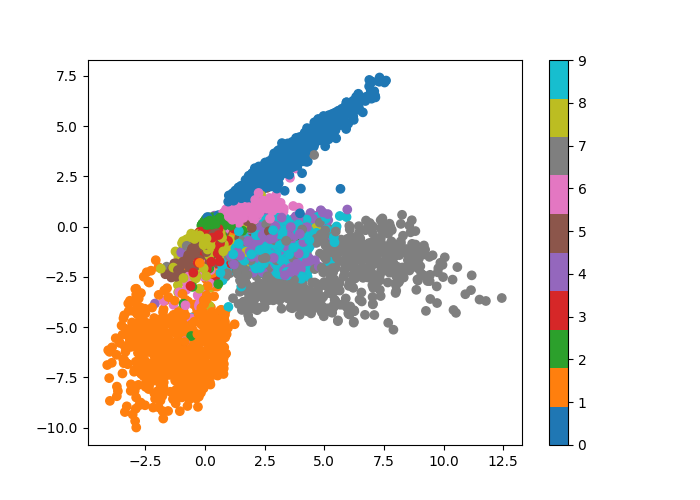
\includegraphics[trim = 10mm 5mm 15mm 10mm, clip, width=\linewidth]{convolutional_VAE_snd_KL_4e-5_10k_epochs_2D_latent}
	\end{minipage}
   \begin{minipage}[b]{0.49\linewidth}
      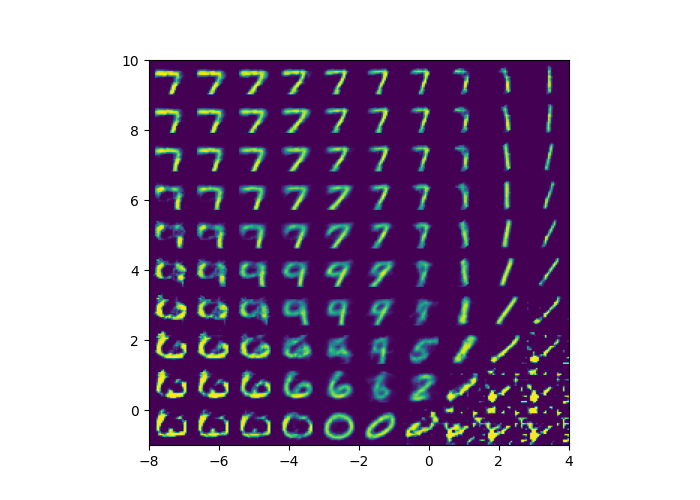
\includegraphics[trim = 15mm 5mm 15mm 10mm, clip, width=\linewidth]{convolutional_VAE_snd_KL_4e-5_10k_epochs_2D_reconstruction}
	\end{minipage}
\end{center}
\caption{On the left-hand side, the figure illustrates the latent space of the variational autoencoder with bottleneck $n_b=2$ and KL-coefficient $\l = \num{4e-5}$, where each dot is a sample from an encoded image of a digit onto a probability density. The color and the corresponding color map represent the digit that was encoded. On the right-hand side the figure illustrates the corresponding reconstruction through the variational autoencoder, where each point of the partitioned  interval $[-4, 8]\times [-6, 6]$ is fed into the decoding architecture of the neural network to generate an image.}\label{fig:convolutional_VAE_snd_KL_4e-5_10k_epochs_2D}
\end{figure}

Another visualisation we want to take a look at is the reconstruction capability of the variational autoencoder. As we did with ordinary autoencoders, we randomly select ten images for each of the ten digits and feed them into the variational autoencoder in order to produce a reconstruction. These reconstructions we can see in Figure \ref{fig:convolutional_VAE_snd_KL_4e-5_10k_epochs_2D_inference}. We can see that the neural network does behave as desired. However, the bottleneck of $n_b=2$ is too small for good reconstructions.

\begin{figure}
\begin{center}
      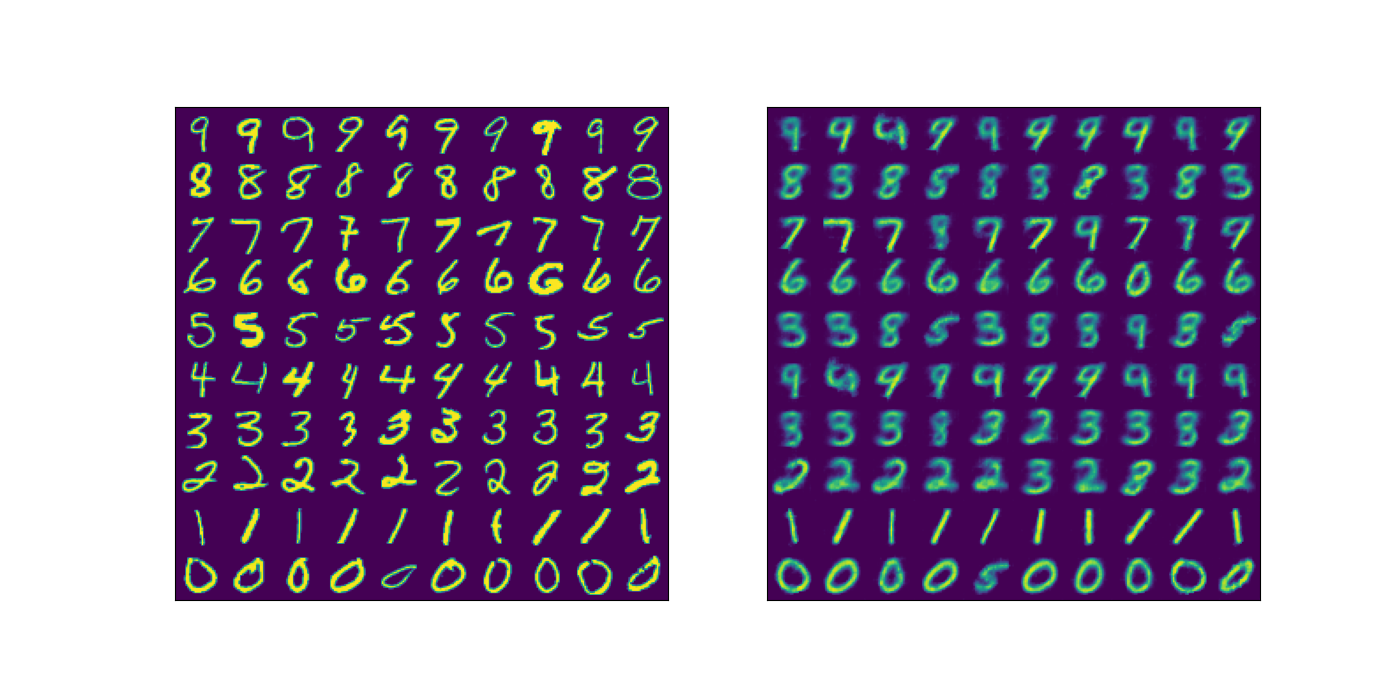
\includegraphics[trim = 15mm 10mm 15mm 15mm, clip, width=\linewidth]{convolutional_VAE_snd_KL_4e-5_10k_epochs_2D_inference}
\end{center}
\caption{On the left-hand side, the figure illustrates $100$ original digits from the MNIST dataset. On the right-hand side, the figure illustrates the same digits after feeding them through the variational autoencoder with bottleneck $n_b=2$ and KL-coefficient $\l = \num{4e-5}$ to produce a reconstruction.}\label{fig:convolutional_VAE_snd_KL_4e-5_10k_epochs_2D_inference}
\end{figure}


Furthermore, we want to take a look at the training progress, which is depicted in Figure \ref{fig:convolutional_VAE_snd_KL_4e-5_10k_epochs_2D_training_progress}. The blue line plots represents the training loss in each epoch and the orange line represents the moving average of the training loss with regard to the 100 surrounding epochs to give an intuition of the trend of the training progress. We see that similarly to the autoencoders, see e.g. Figure \ref{fig:linear_AE_2d_adam_training_progress}, the training loss first falls rapidly and then after roughly $1000$ epochs barely changes.

\begin{figure}
\begin{center}
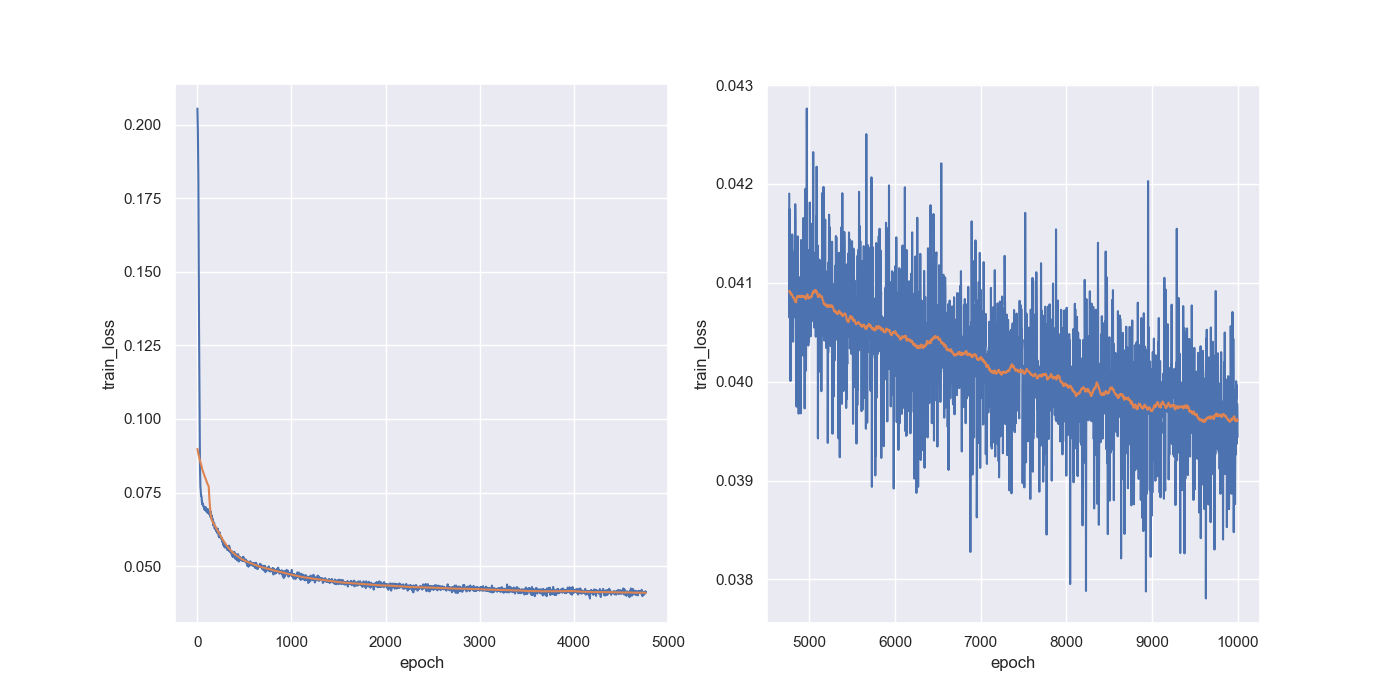
\includegraphics[width=\linewidth]{convolutional_VAE_snd_KL_4e-5_10k_epochs_2D_training_progress}
\end{center}
\caption{The figure illustrates the training progresses of the variational autoencoder with bottleneck $n_b=2$ and KL-coefficient $\l = \num{4e-5}$ with epochs on one axis and corresponding training loss on the other axis. On the left side we see the first $3.500$ epochs and on the right side the following epochs until $10.000$. The blue line represents the loss in each epoch and the orange line represents the moving average over $100$ epochs to point out the trend of the training progress.}\label{fig:convolutional_VAE_snd_KL_4e-5_10k_epochs_2D_training_progress}
\end{figure}


Lastly, we visualise the reconstruction errors of the neural network similarly as we did in Chapter~\ref{chap:ae}. For each of the ten digits we compute the average Euclidean distance between reconstruction and original image over the entire dataset. These reconstruction errors we portray in Figure \ref{fig:convolutional_VAE_snd_KL_4e-5_10k_epochs_2D_errors}. We can see that as with the discriminative model, a bottleneck dimension of $n_b=2$ is too small to produce good reconstructions. Therefore, the resulting reconstruction error is similar for both neural networks.


\begin{figure}
\begin{center}
      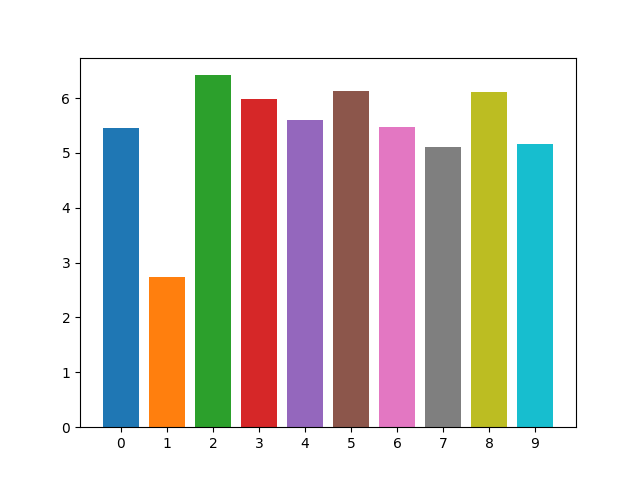
\includegraphics[width=0.49\linewidth]{convolutional_VAE_snd_KL_4e-5_10k_epochs_2D_errors}
\end{center}
\caption{The figure illustrates the test errors of the variational autoencoder with bottleneck $n_b=2$ and KL-coefficient $\l = \num{4e-5}$, where each bar represents the averaged test errors over the entire MNIST dataset for each of the ten digits.}\label{fig:convolutional_VAE_snd_KL_4e-5_10k_epochs_2D_errors}
\end{figure}


Even though we can see that the training of the variational autoencoder was successful, a bottleneck of $n_b=2$ dimensions is simply too small for the network to produce good reconstructions. For this reason, we want to increase the bottleneck to $n_b=3$ and consider its latent space as well as the reconstructions. Since the training progress looks similar to the two-dimensional case, we omit its depiction here and instead kindly refer to the Python code appended to this thesis.\\
Having trained the variational autoencoder with bottleneck $n_b=3$, we depict the latent space from two different perspectives in Figure \ref{fig:convolutional_VAE_snd_KL_4e-5_10k_epochs_3D_latent}. We can see that the clusters of each digit are well separated for digits that look differently, e.g. the digits $1$ and $0$ form clear clusters. However, digits that look similar, e.g. $4$ and $9$ are not separated at all and are mapped onto the same region in the latent space. This will affect the reconstructions, which we can see in Figure \ref{fig:convolutional_VAE_snd_KL_4e-5_10k_epochs_3D_inference}. In this figure we can see, as in the two dimensional case, on the left-hand side $100$ samples from the MNIST dataset, where we randomly chose $10$ sampels for each of the ten digits. On the right-hand side we can see the corresponding reconstructions produced by the network. As anticipated, the digits which are well separated are reconstructed quite well, e.g. $0$, $1$ and $7$, whereas the digits that are not separated at all can hardly be distinguished, e.g. $4$ and $9$.


\begin{figure}
\begin{center}
   \begin{minipage}[b]{0.49\linewidth}
      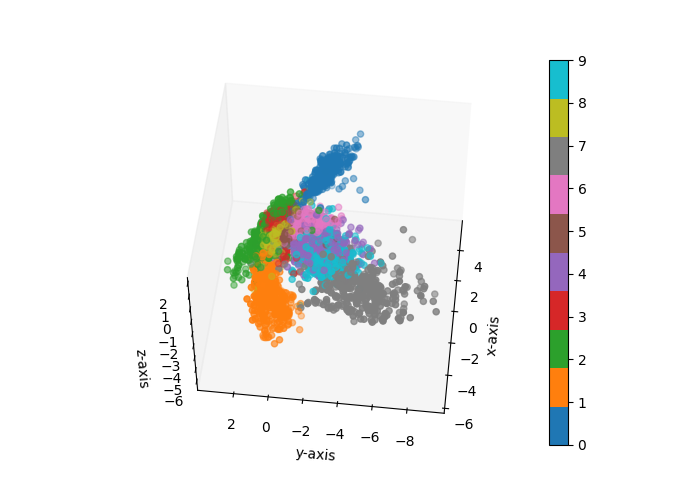
\includegraphics[trim = 20mm 10mm 20mm 10mm, clip, width=\linewidth]{convolutional_VAE_snd_KL_4e-5_10k_epochs_3D_latent_1}
	\end{minipage}
   \begin{minipage}[b]{0.49\linewidth}
      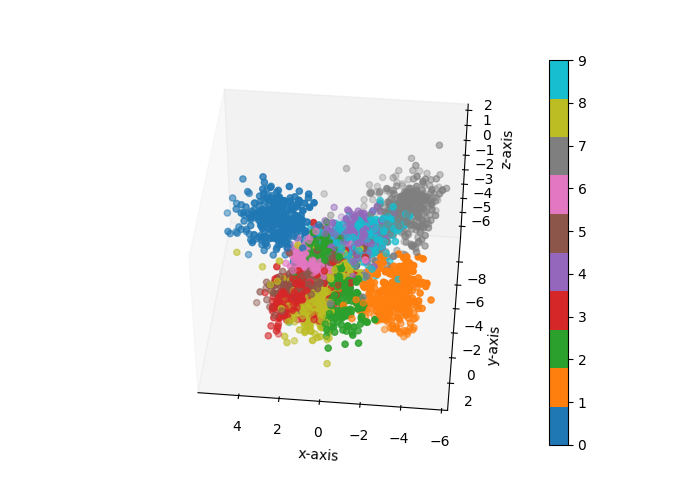
\includegraphics[trim = 20mm 10mm 20mm 10mm, clip, width=\linewidth]{convolutional_VAE_snd_KL_4e-5_10k_epochs_3D_latent_2}
	\end{minipage}
\end{center}
\caption{The figure illustrates the latent space of the variational autoencoder with bottleneck $n_b=3$ and KL-coefficient $\l = \num{4e-5}$ from two different perspectives. Each dot is a sample from the encoded image of a digit onto a probability density. The color and the corresponding color map represent the digit that was encoded.}\label{fig:convolutional_VAE_snd_KL_4e-5_10k_epochs_3D_latent}
\end{figure}


\begin{figure}
\begin{center}
      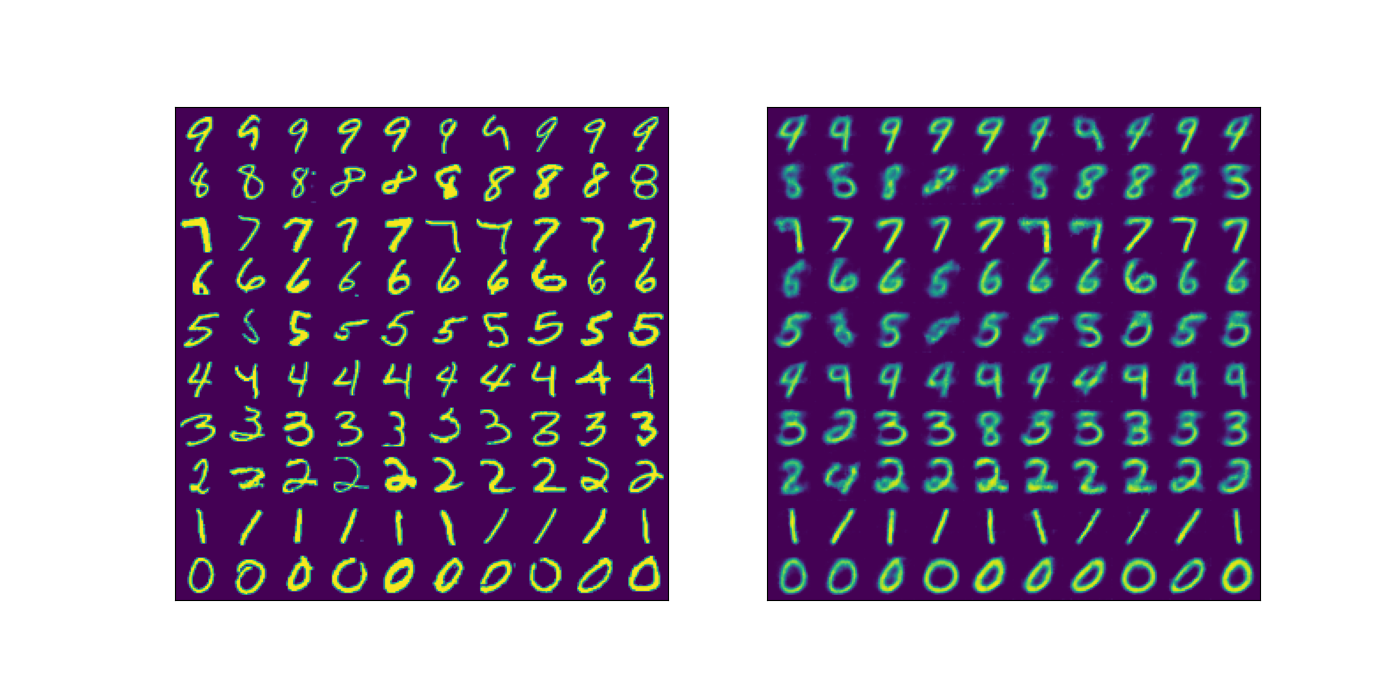
\includegraphics[trim = 15mm 10mm 15mm 15mm, clip, width=\linewidth]{convolutional_VAE_snd_KL_4e-5_10k_epochs_3D_inference}
\end{center}
\caption{On the left-hand side, the figure illustrates $100$ original digits from the MNIST dataset. On the right-hand side, the figure illustrates the same digits after feeding them through the variational autoencoder with bottleneck $n_b=3$ and KL-coefficient $\l = \num{4e-5}$ to produce a reconstruction.}\label{fig:convolutional_VAE_snd_KL_4e-5_10k_epochs_3D_inference}
\end{figure}


Lastly, we visualise the reconstruction errors in Figure \ref{fig:convolutional_VAE_snd_KL_4e-5_10k_epochs_3D_errors}. We can see that the errors are slightly smaller comparing to the $2$-dimensional case, see Figure \ref{fig:convolutional_VAE_snd_KL_4e-5_10k_epochs_2D_errors}.



\begin{figure}
\begin{center}
      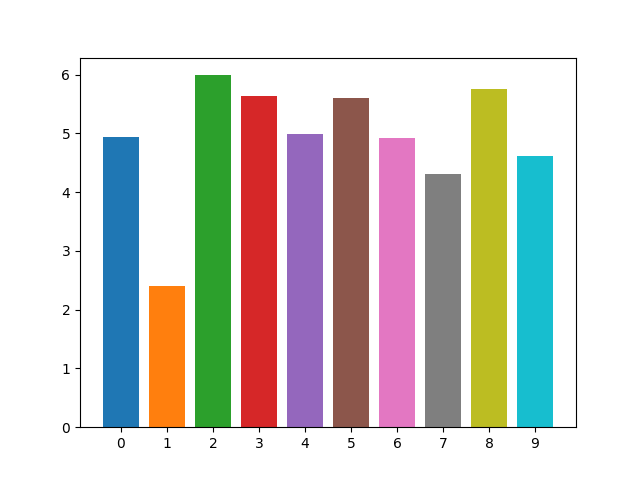
\includegraphics[width=0.49\linewidth]{convolutional_VAE_snd_KL_4e-5_10k_epochs_3D_errors}
\end{center}
\caption{The figure illustrates the test errors of the variational autoencoder with bottleneck $n_b=3$ and KL-coefficient $\l = \num{4e-5}$, where each bar represents the averaged test errors over the entire MNIST dataset for each of the ten digits.}\label{fig:convolutional_VAE_snd_KL_4e-5_10k_epochs_3D_errors}
\end{figure}


Furthermore, to be able to compare the reconstruction capability of the convolutional autoencoder, see Figure \ref{fig:convolutional_AE_inference}, to the variational autoencoder in a sensible way, we now want to increase the bottleneck dimension to $n_b=64$ and depict its reconstructions. These we can see in Figure \ref{fig:convolutional_VAE_snd_KL_4e-5_10k_epochs_64D_inference}. We can see that the reconstructions of the variational autoencoder are slightly worse than compared to the convolutional autoencoder.

\begin{figure}
\begin{center}
      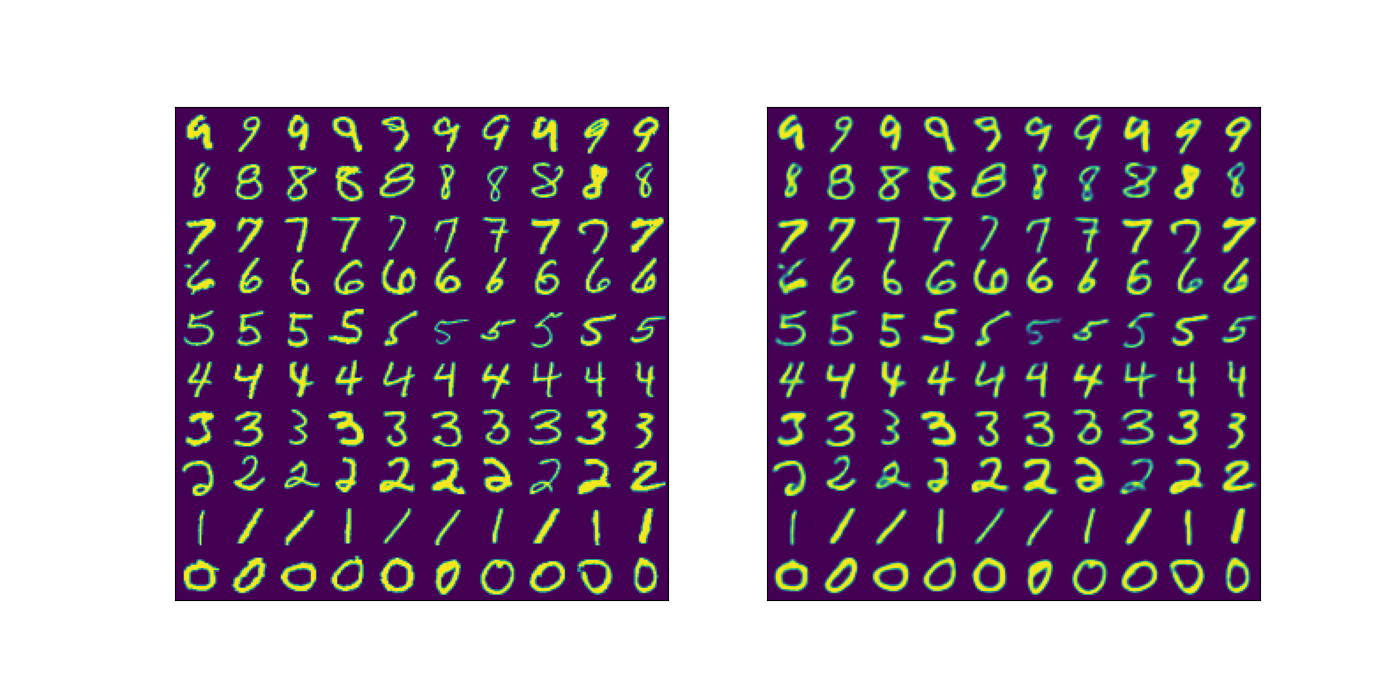
\includegraphics[trim = 15mm 10mm 15mm 15mm, clip, width=\linewidth]{convolutional_VAE_snd_KL_4e-5_10k_epochs_64D_inference}
\end{center}
\caption{On the left-hand side, the figure illustrates $100$ original digits from the MNIST dataset. On the right-hand side, the figure illustrates the same digits after feeding them through the variational autoencoder with bottleneck $n_b=64$ and KL-coefficient $\l = \num{4e-5}$ to produce a reconstruction.}\label{fig:convolutional_VAE_snd_KL_4e-5_10k_epochs_64D_inference}
\end{figure}


Moreover, we portray the reconstruction errors in Figure \ref{fig:convolutional_VAE_snd_KL_4e-5_10k_epochs_64D_errors}. Here we can see as well, that the reconstruction errors for the variational autoencoder are slightly higher than compared to the convolutional autoencoder, see Figure \ref{fig:convolutional_AE_errors}. This is due to the fact that producing single point evaluations, which these reconstructions essentially are, are tasks that discriminative models are tailored for. Therefore, the convolutional autoencoder performs slightly better. However, if we want to generate new samples, e.g. by adding some noise onto an encoded representation, the variational autoencoder performs much better. To prove this, we randomly chose one sample for each digit and then add some $\mathcal{N}(0, 1)$-noise onto the encoding. Then we reconstruct the images with the help of the corresponding decoding architectures of each neural network. These newly generated samples we depict in Figure \ref{fig:convolutional_VAE_vs_convolutional_AE}, where on the left-hand side we can see the generated samples for the variational autoencoder and on the right-hand side for the convolutional autoencoder.

\begin{figure}
\begin{center}
      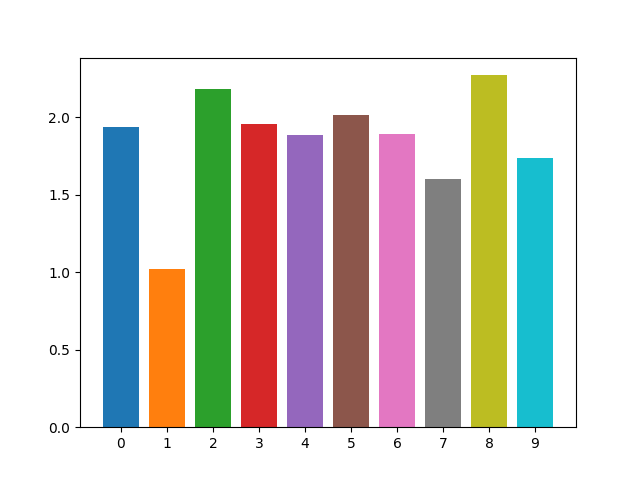
\includegraphics[width=0.49\linewidth]{convolutional_VAE_snd_KL_4e-5_10k_epochs_64D_errors}
\end{center}
\caption{The figure illustrates the test errors of the variational autoencoder with bottleneck $n_b=64$ and KL-coefficient $\l = \num{4e-5}$, where each bar represents the averaged test errors over the entire MNIST dataset for each of the ten digits.}\label{fig:convolutional_VAE_snd_KL_4e-5_10k_epochs_64D_errors}
\end{figure}


\begin{figure}
\begin{center}
\begin{minipage}[b]{0.49\linewidth}
      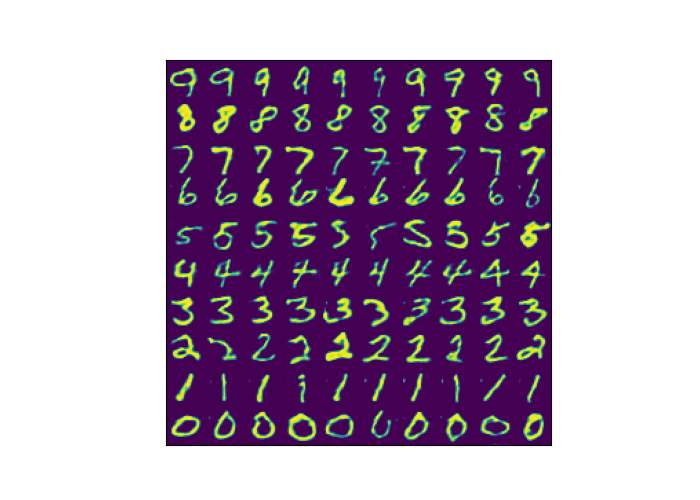
\includegraphics[trim = 15mm 10mm 15mm 10mm, clip, width=\linewidth]{convolutional_VAE_snd_KL_4e-5_10k_epochs_64D_generated}
	\end{minipage}
   \begin{minipage}[b]{0.49\linewidth}
      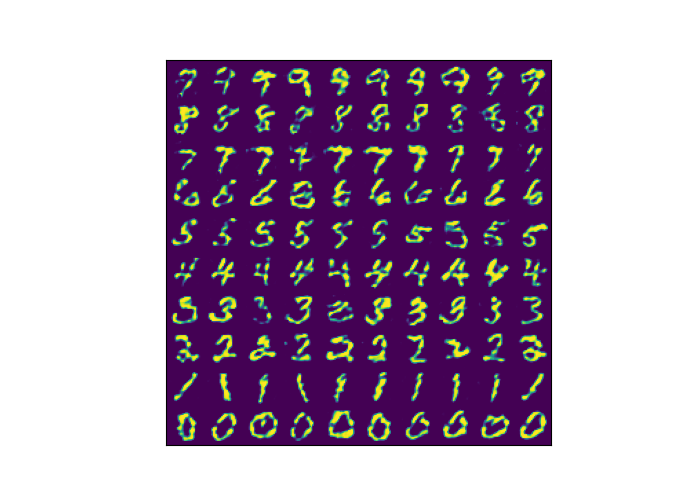
\includegraphics[trim = 15mm 10mm 15mm 10mm, clip, width=\linewidth]{convolutional_AE_generated}
	\end{minipage}
\end{center}
\caption{On the left-hand side, the figure illustrates $100$ generated samples by the variational autoencoder with bottleneck $n_b=64$. On the right-hand side, the figure illustrates $100$ generated samples by the convolutional autoencoder witch bottleneck $n_b=64$ as well.}\label{fig:convolutional_VAE_vs_convolutional_AE}
\end{figure}


We can clearly see that the variational autoencoder is much more stable when applying noise onto the encoded representations and thus, generates much better samples. At this point it is worth mentioning that there indeed are some generated images that do not look as good as other ones. This is due to the fact that we simply chose an arbitrary sample from the data set to begin with. If we were to first determine the cluster center, by e.g. averaging the mean over a certain number of samples, then the generation would be much more stable. This we do in Figure \ref{fig:convolutional_VAE_better_generations}.


\begin{figure}
\begin{center}
   \begin{minipage}[b]{0.60\linewidth}
      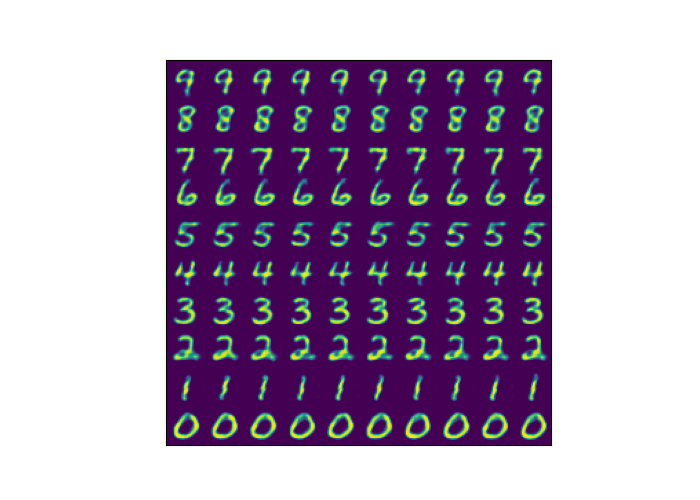
\includegraphics[trim = 15mm 10mm 15mm 10mm, clip, width=\linewidth]{convolutional_VAE_snd_KL_4e-5_10k_epochs_64D_generated_optimal}
	\end{minipage}
\end{center}
\caption{The figure illustrates $100$ generated samples by the variational autoencoder with bottleneck $n_b=64$. To make the generation more stable, we first averaged the encoded means and variances over all digits in the dataset and afterwards applied some noise to the averaged mean.}\label{fig:convolutional_VAE_better_generations}
\end{figure}


We now have considered some variational autoencoders with different bottleneck dimensions. However, we always chose the KL-coefficient to be $\l = \num{4e-5}$, which is comparatively small. We now want to analyse the influence of the said coefficient on the resulting variational autoencoder. We begin by increasing the coefficient to $\l = \num{4e-4}$. The corresponding latent space is illustrated in Figure \ref{fig:convolutional_VAE_snd_KL_4e-4_5k_epochs_3D_latent}. We can see that the clusters are much more ball shaped than with the lower KL-coefficient, see Figure \ref{fig:convolutional_VAE_snd_KL_4e-5_10k_epochs_3D_latent}. This phenomenon is a consequence of the normal distributed density, which the samples are encoded to.

\begin{figure}
\begin{center}
   \begin{minipage}[b]{0.49\linewidth}
      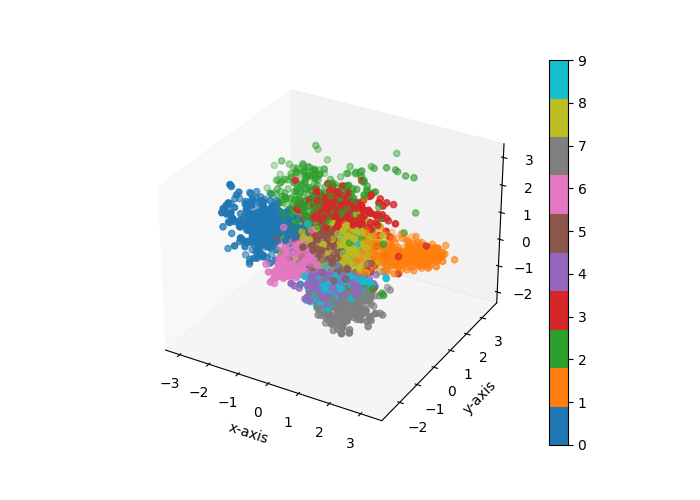
\includegraphics[trim = 20mm 10mm 20mm 10mm, clip, width=\linewidth]{convolutional_VAE_snd_KL_4e-4_5k_epochs_3D_latent_1}
	\end{minipage}
   \begin{minipage}[b]{0.49\linewidth}
      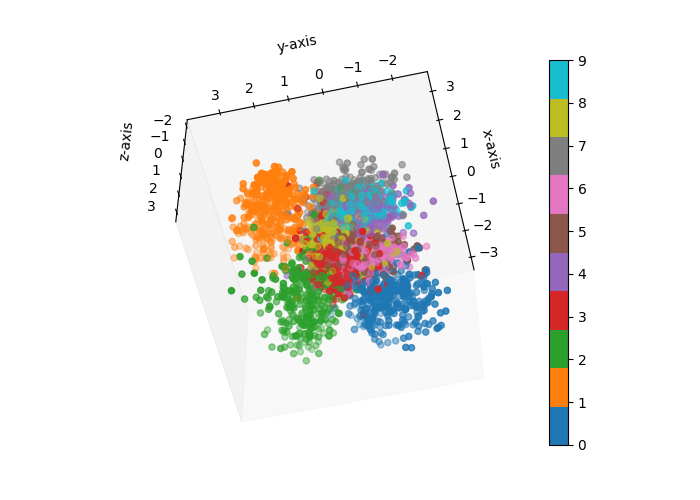
\includegraphics[trim = 20mm 10mm 20mm 10mm, clip, width=\linewidth]{convolutional_VAE_snd_KL_4e-4_5k_epochs_3D_latent_2}
	\end{minipage}
\end{center}
\caption{The figure illustrates the latent space of the variational autoencoder with bottleneck $n_b=3$ and KL-coefficient $\l = \num{4e-4}$ from two different perspectives. Each dot is a sample from the encoded image of a digit onto a probability density. The color and the corresponding color map represent the digit that was encoded.}\label{fig:convolutional_VAE_snd_KL_4e-4_5k_epochs_3D_latent}
\end{figure}


If we now take a look at the reconstructions of the variational autoencoder, see Figure \ref{fig:convolutional_VAE_snd_KL_4e-4_5k_epochs_3D_inference}, we see that they still are not good, even though they are a little smoother than compared to the $\l = \num{4e-5}$ case.
Moreover, we illustrate the reconstruction errors in Figure \ref{fig:convolutional_VAE_snd_KL_4e-4_5k_epochs_3D_errors}. We highlight, that the result is that the tradeof for a smoother latent space is a higher reconstruction error.


\begin{figure}
\begin{center}
      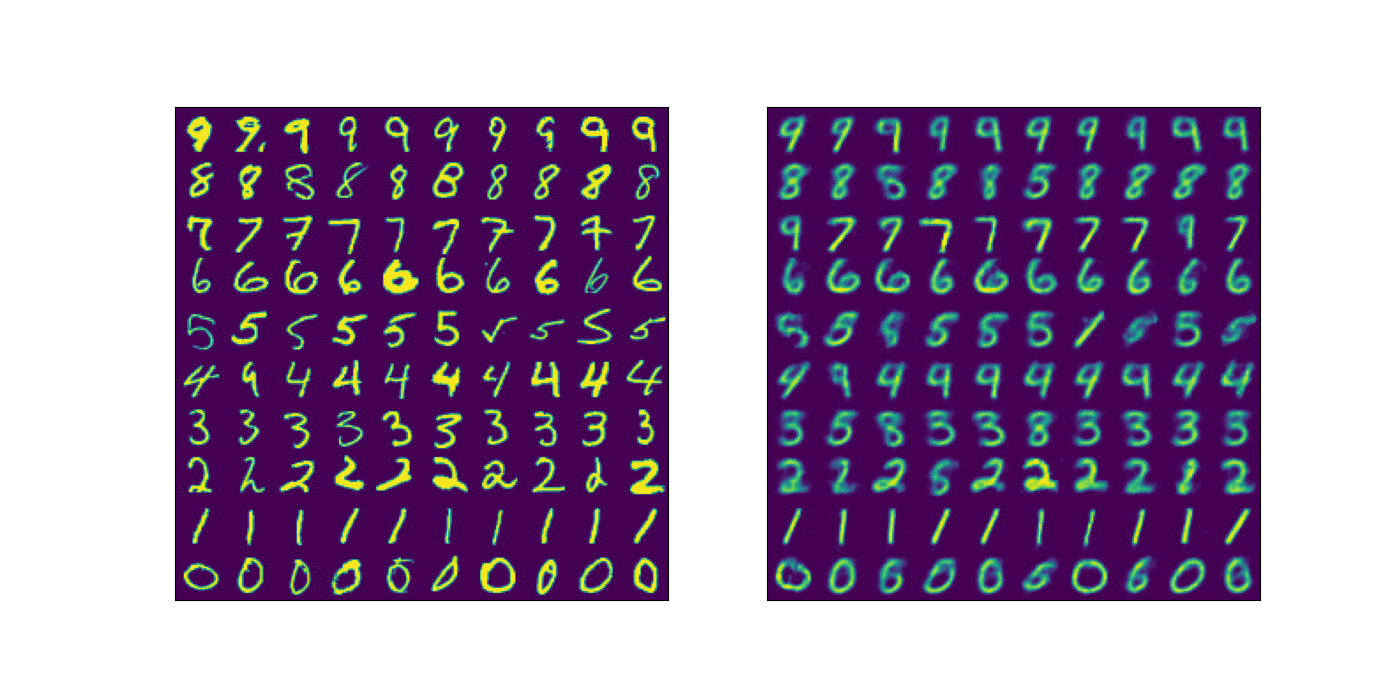
\includegraphics[trim = 15mm 10mm 15mm 15mm, clip, width=\linewidth]{convolutional_VAE_snd_KL_4e-4_5k_epochs_3D_inference}
\end{center}
\caption{On the left-hand side, the figure illustrates $100$ original digits from the MNIST dataset. On the right-hand side, the figure illustrates the same digits after feeding them through the variational autoencoder with bottleneck $n_b=3$ and KL-coefficient $\l=\num{4e-4}$ to produce a reconstruction.}\label{fig:convolutional_VAE_snd_KL_4e-4_5k_epochs_3D_inference}
\end{figure}


\begin{figure}
\begin{center}
      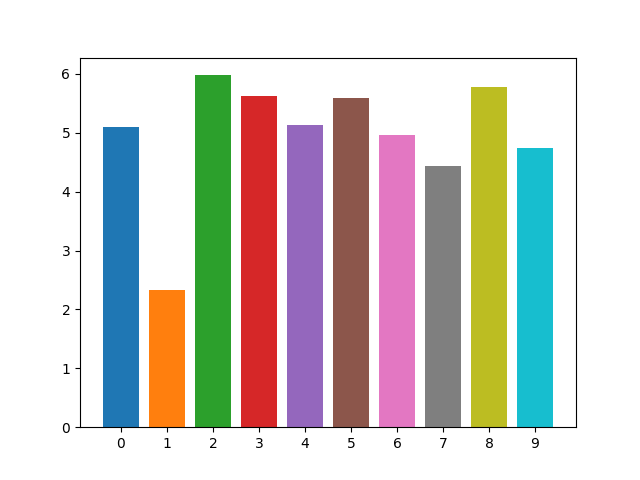
\includegraphics[width=0.49\linewidth]{convolutional_VAE_snd_KL_4e-4_5k_epochs_3D_errors}
\end{center}
\caption{The figure illustrates the test errors of the variational autoencoder with bottleneck $n_b=3$ and KL-coefficient $\l = \num{4e-4}$, where each bar represents the averaged test errors over the entire MNIST dataset for each of the ten digits.}\label{fig:convolutional_VAE_snd_KL_4e-4_5k_epochs_3D_errors}
\end{figure}


We proceed to increase the KL-coefficient even further and consider the case $\l = \num{4e-2}$. This is a very interesting example for different reasons. The first reason is that if we take a look at the latent space of this variational autoencoder, see Figure \ref{fig:convolutional_VAE_snd_KL_4e-2_10k_epochs_3D_latent}, we realise that every digit is encoded onto a $3$-dimensional normal distribution with basically the same density function. There can not be determined a single cluster. Therefore, the reconstructions, see Figure \ref{fig:convolutional_VAE_snd_KL_4e-2_10k_epochs_3D_inference}, can not be identified as digits either. The reconstruction error, see Figure \ref{fig:convolutional_VAE_snd_KL_4e-2_10k_epochs_3D_errors}, is quite high and pretty similar for all ten digits.

\begin{figure}
\begin{center}
   \begin{minipage}[b]{0.49\linewidth}
      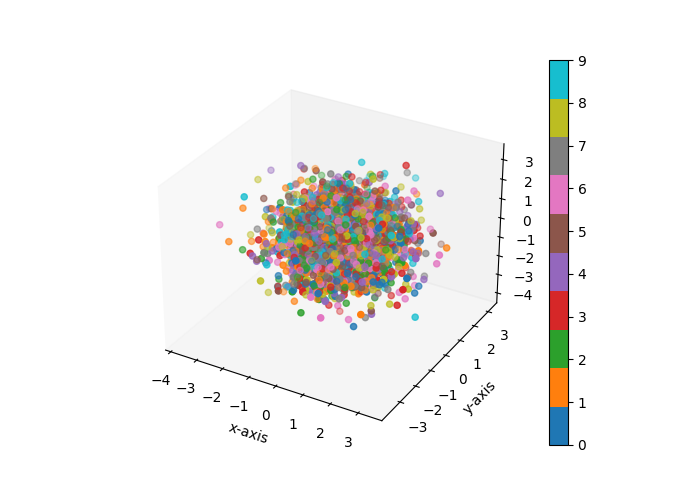
\includegraphics[trim = 20mm 10mm 20mm 10mm, clip, width=\linewidth]{convolutional_VAE_snd_KL_4e-2_10k_epochs_3D_latent_1}
	\end{minipage}
   \begin{minipage}[b]{0.49\linewidth}
      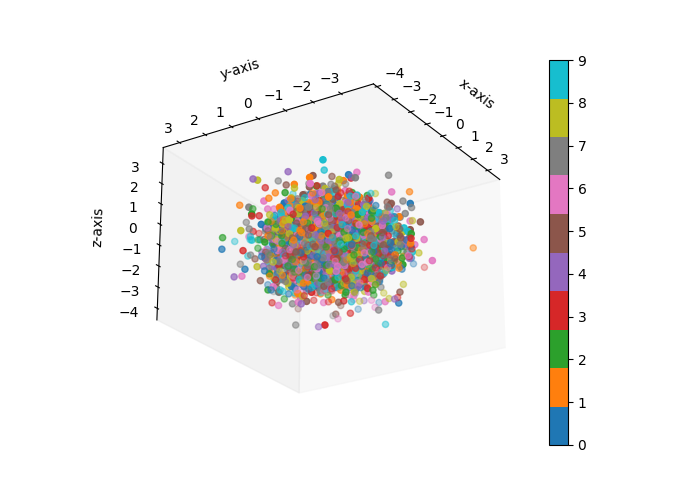
\includegraphics[trim = 20mm 10mm 20mm 10mm, clip, width=\linewidth]{convolutional_VAE_snd_KL_4e-2_10k_epochs_3D_latent_2}
	\end{minipage}
\end{center}
\caption{The figure illustrates the latent space of the variational autoencoder with bottleneck $n_b=3$ and KL-coefficient $\l = \num{4e-2}$ from two different perspectives. Each dot is a sample from the encoded image of a digit onto a probability density. The color and the corresponding color map represent the digit that was encoded.}\label{fig:convolutional_VAE_snd_KL_4e-2_10k_epochs_3D_latent}
\end{figure}


\begin{figure}
\begin{center}
      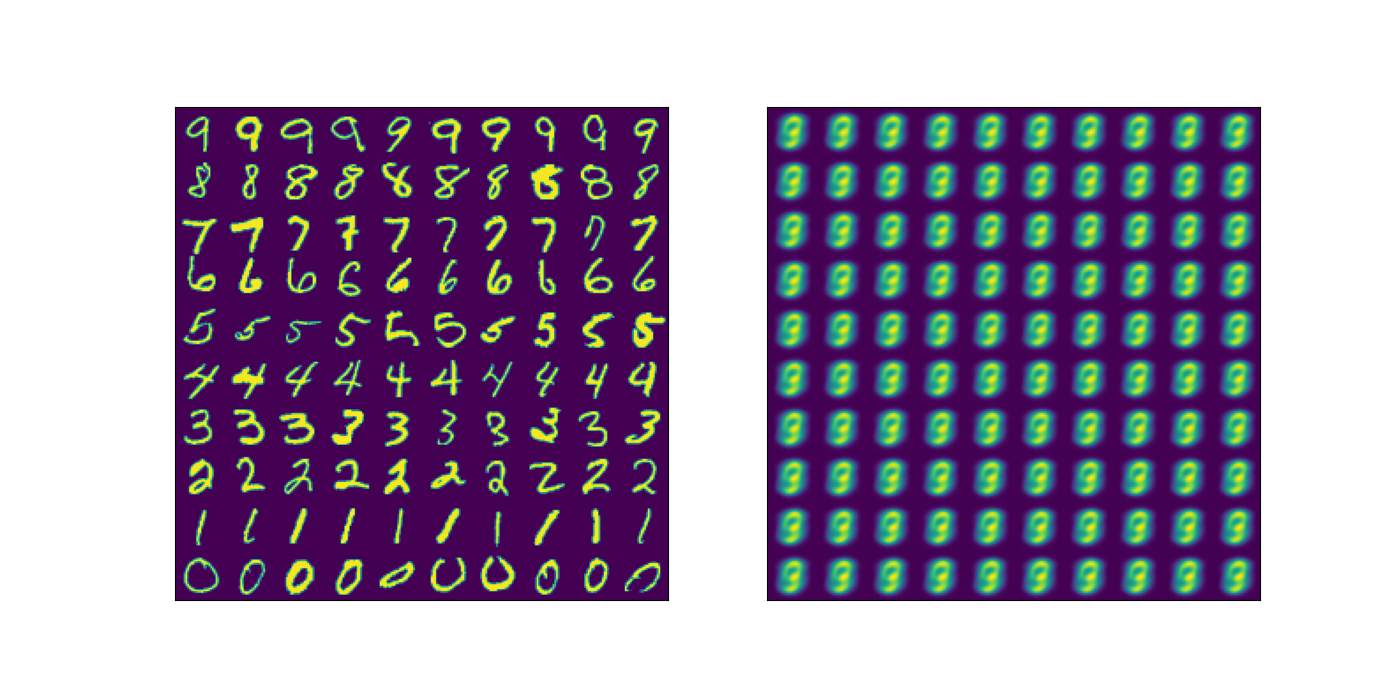
\includegraphics[trim = 15mm 10mm 15mm 15mm, clip, width=\linewidth]{convolutional_VAE_snd_KL_4e-2_10k_epochs_3D_inference}
\end{center}
\caption{On the left-hand side, the figure illustrates $100$ original digits from the MNIST dataset. On the right-hand side, the figure illustrates the same digits after feeding them through the variational autoencoder with bottleneck $n_b=3$ and KL-coefficient $\l=\num{4e-2}$ to produce a reconstruction.}\label{fig:convolutional_VAE_snd_KL_4e-2_10k_epochs_3D_inference}
\end{figure}


\begin{figure}
\begin{center}
      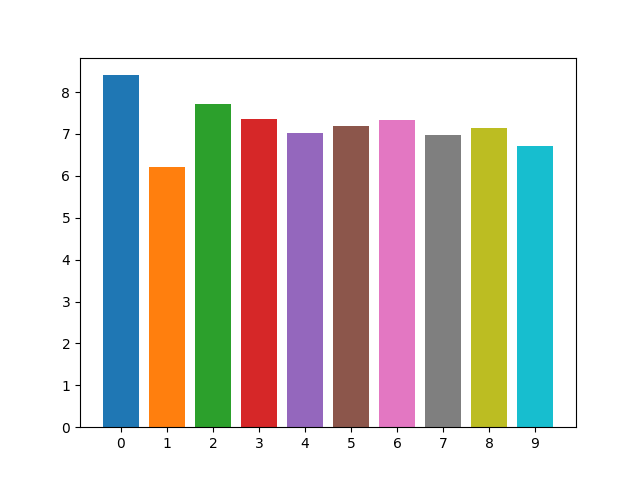
\includegraphics[width=0.49\linewidth]{convolutional_VAE_snd_KL_4e-2_10k_epochs_3D_errors}
\end{center}
\caption{The figure illustrates the test errors of the variational autoencoder with bottleneck $n_b=3$ and KL-coefficient $\l = \num{4e-2}$, where each bar represents the averaged test errors over the entire MNIST dataset for each of the ten digits.}\label{fig:convolutional_VAE_snd_KL_4e-2_10k_epochs_3D_errors}
\end{figure}


However, if we increase the bottleneck to $n_b=10$, the reconstructions, see Figure \ref{fig:convolutional_VAE_snd_KL_4e-2_10k_epochs_10D_inference} are recognizable again. This means that if the network has enough \glqq spare dimensions\grqq{} it can find itself a mapping such that the encodings form clusters in the latent space. The reconstruction error, see Figure \ref{fig:convolutional_VAE_new_idea_KL_4e-2_10k_epochs_10D_errors}, is again comparatively small, which verifies the fact that the neural network encodes the samples onto distinct densities now.

\begin{figure}
\begin{center}
      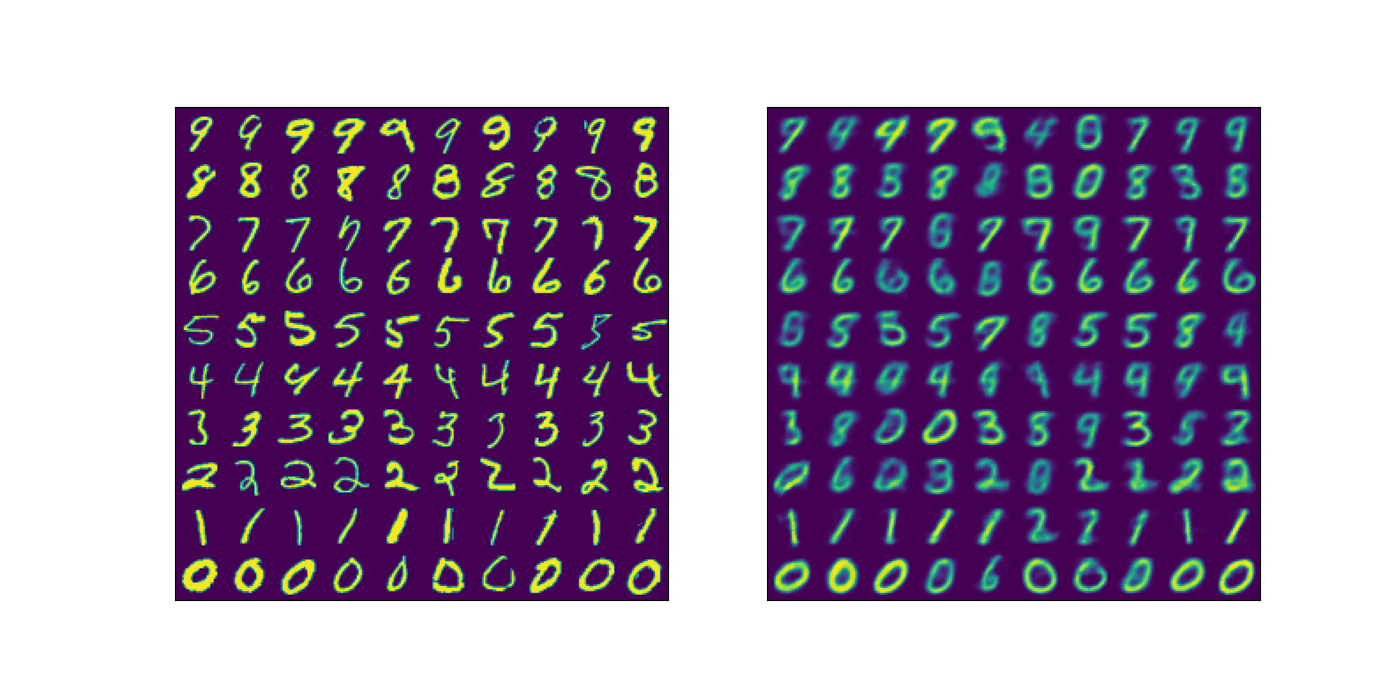
\includegraphics[trim = 15mm 10mm 15mm 15mm, clip, width=\linewidth]{convolutional_VAE_snd_KL_4e-2_10k_epochs_10D_inference}
\end{center}
\caption{On the left-hand side, the figure illustrates $100$ original digits from the MNIST dataset. On the right-hand side, the figure illustrates the same digits after feeding them through the variational autoencoder with bottleneck $n_b=10$ and KL-coefficient $\l=\num{4e-2}$ to produce a reconstruction.}\label{fig:convolutional_VAE_snd_KL_4e-2_10k_epochs_10D_inference}
\end{figure}


\begin{figure}
\begin{center}
      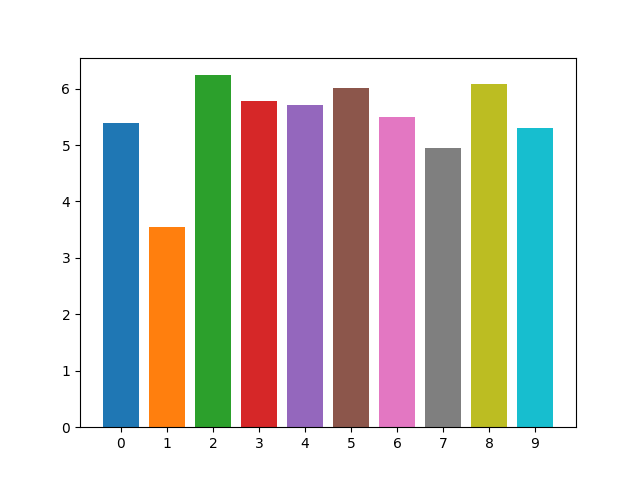
\includegraphics[width=0.49\linewidth]{convolutional_VAE_snd_KL_4e-2_10k_epochs_10D_errors}
\end{center}
\caption{The figure illustrates the test errors of the variational autoencoder with bottleneck $n_b=10$ and KL-coefficient $\l = \num{4e-2}$, where each bar represents the averaged test errors over the entire MNIST dataset for each of the ten digits.}\label{fig:convolutional_VAE_snd_KL_4e-2_10k_epochs_10D_errors}
\end{figure}


If we now increase the bottleneck to $n_b=64$, see Figure \ref{fig:convolutional_VAE_snd_KL_4e-2_10k_epochs_64D_inference}, we realise that the reconstructions are quite good and hence, the neural network behaves as it is supposed to. Moreover, taking a look at the reconstruction error, see Figure \ref{fig:convolutional_VAE_snd_KL_4e-2_10k_epochs_64D_inference} supports this claim.

\begin{figure}
\begin{center}
      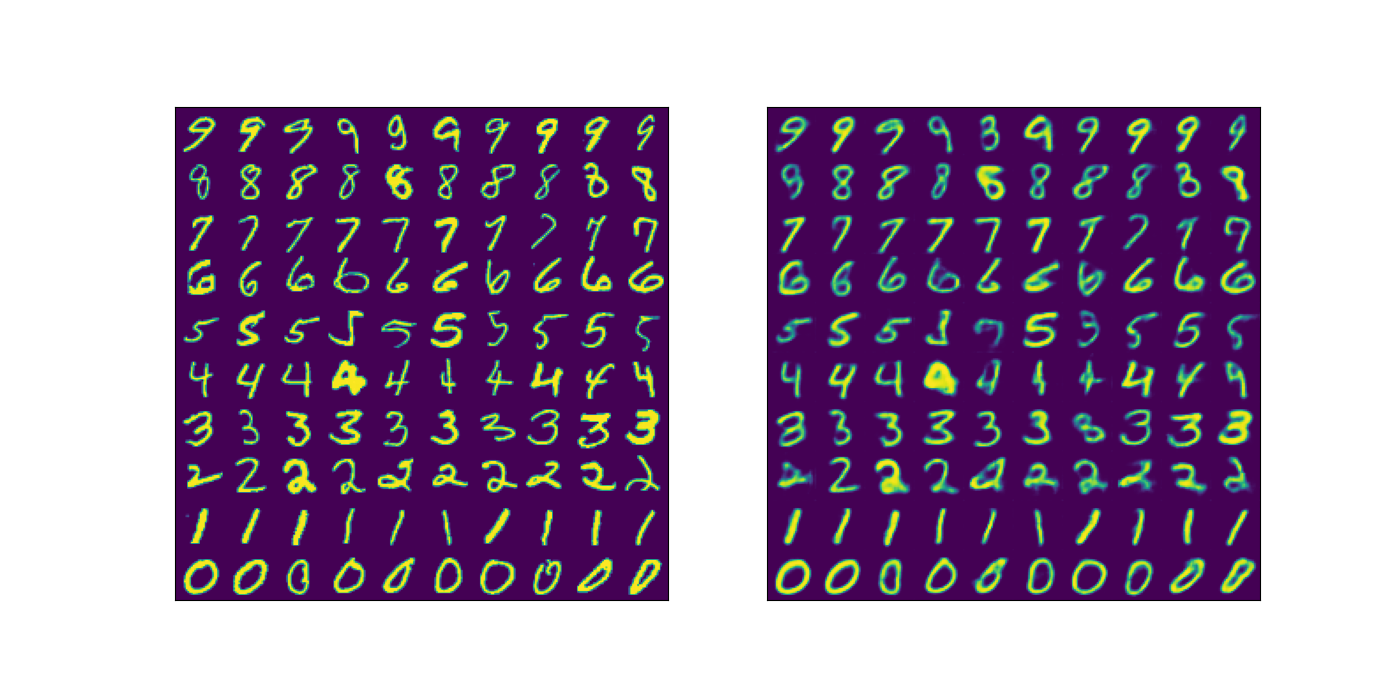
\includegraphics[trim = 15mm 10mm 15mm 15mm, clip, width=\linewidth]{convolutional_VAE_snd_KL_4e-2_10k_epochs_64D_inference}
\end{center}
\caption{On the left-hand side, the figure illustrates $100$ original digits from the MNIST dataset. On the right-hand side, the figure illustrates the same digits after feeding them through the variational autoencoder with bottleneck $n_b=64$ and KL-coefficient $\l=\num{4e-2}$ to produce a reconstruction.}\label{fig:convolutional_VAE_snd_KL_4e-2_10k_epochs_64D_inference}
\end{figure}

\begin{figure}
\begin{center}
      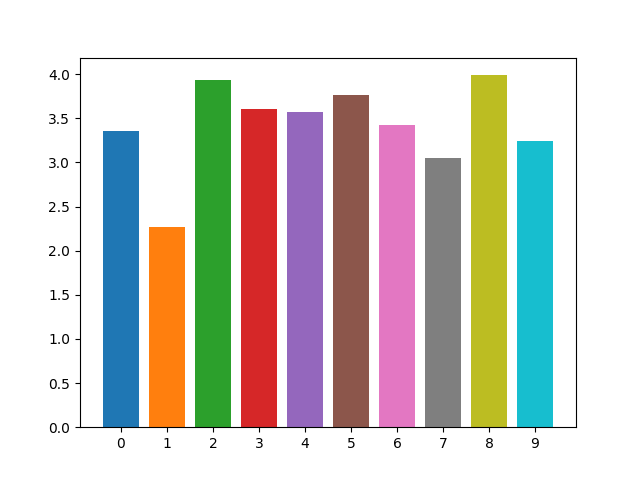
\includegraphics[width=0.49\linewidth]{convolutional_VAE_snd_KL_4e-2_10k_epochs_64D_errors}
\end{center}
\caption{The figure illustrates the test errors of the variational autoencoder with bottleneck $n_b=64$ and KL-coefficient $\l = \num{4e-2}$, where each bar represents the averaged test errors over the entire MNIST dataset for each of the ten digits.}\label{fig:convolutional_VAE_snd_KL_4e-2_10k_epochs_64D_errors}
\end{figure}


As the last experiment we want to analyse a slightly different approach than proposed in literature. As previously described, the common approach in literature is to chose the posterior to be a standard normal distribution and allow the neural network to find a latent representation such that the encoded densities are close to a standard normal distribution but still differ enough to form clusters for each of the encoded digits. We now propose the following. Since we know that we have ten digits and thus, will have ten clusters in the latent space, we define for each of the digits a different vector which will be the mean of its chosen posterior density. This way, we can force the neural network to spatially separate the clusters. We depict the resulting latent space for a variational autoencoder with bottleneck $n_b=3$ and KL-coefficient $\l=\num{4e-2}$ in Figure \ref{fig:convolutional_VAE_new_idea_KL_4e-2_10k_epochs_3D_latent}.

\begin{figure}
\begin{center}
   \begin{minipage}[b]{0.49\linewidth}
      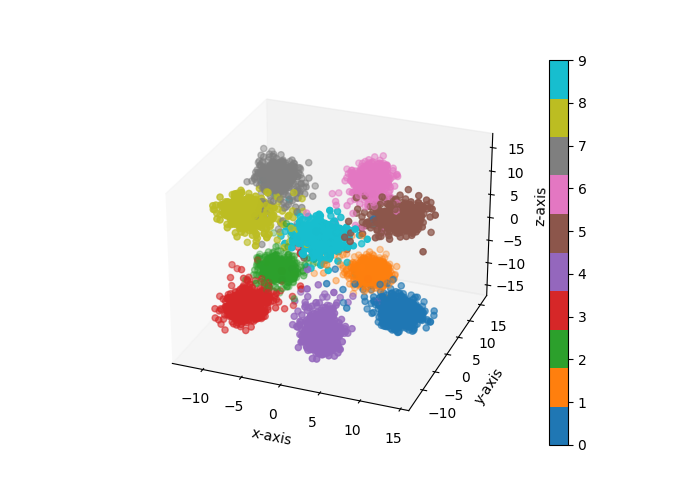
\includegraphics[trim = 20mm 10mm 20mm 10mm, clip, width=\linewidth]{convolutional_VAE_new_idea_KL_4e-2_10k_epochs_3D_latent_1}
	\end{minipage}
   \begin{minipage}[b]{0.49\linewidth}
      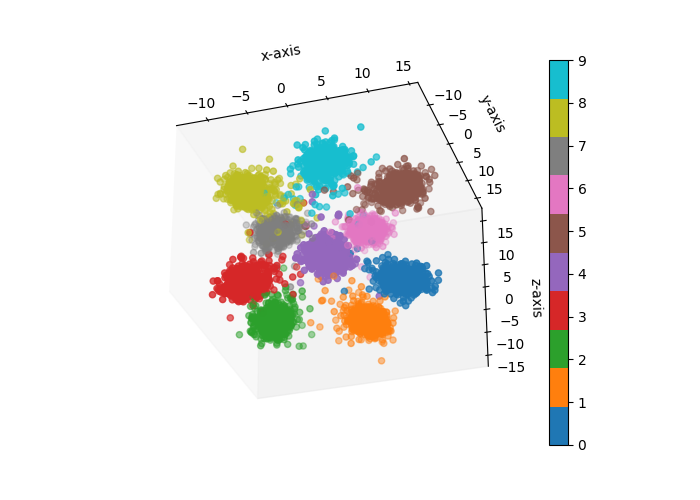
\includegraphics[trim = 20mm 10mm 20mm 10mm, clip, width=\linewidth]{convolutional_VAE_new_idea_KL_4e-2_10k_epochs_3D_latent_2}
	\end{minipage}
\end{center}
\caption{The figure illustrates the latent space of the variational autoencoder with the posterior chosen customly, where we choose the bottleneck $n_b=3$ and KL-coefficient $\l = \num{4e-2}$, from two different perspectives. Each dot is a sample from the encoded image of a digit onto a probability density. The color and the corresponding color map represent the digit that was encoded.}\label{fig:convolutional_VAE_new_idea_KL_4e-2_10k_epochs_3D_latent}
\end{figure}

Furthermore, we visualise the reconstructions for each digit in Figure \ref{fig:convolutional_VAE_new_idea_KL_4e-2_10k_epochs_3D_inference} and the corresponding reconstruction errors in Figure \ref{fig:convolutional_VAE_new_idea_KL_4e-2_10k_epochs_3D_errors}.


\begin{figure}
\begin{center}
      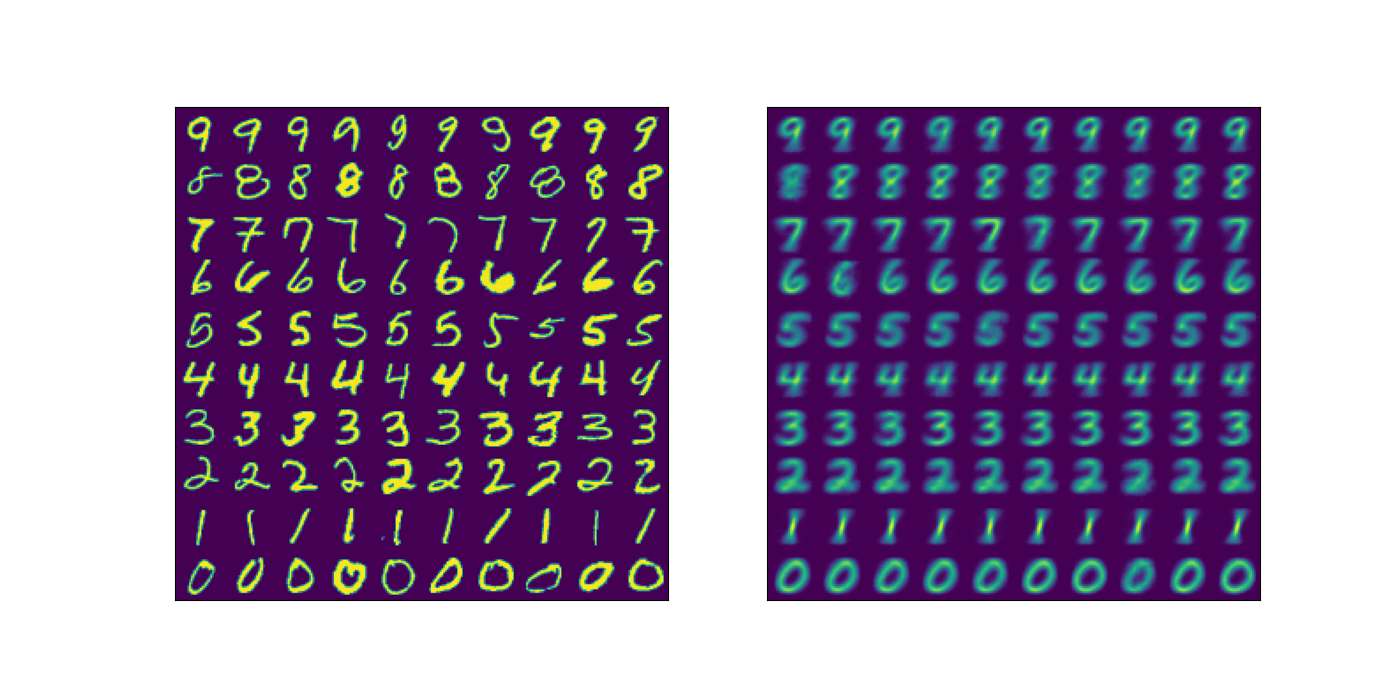
\includegraphics[trim = 15mm 10mm 15mm 15mm, clip, width=\linewidth]{convolutional_VAE_new_idea_KL_4e-2_10k_epochs_3D_inference}
\end{center}
\caption{On the left-hand side, the figure illustrates $100$ original digits from the MNIST dataset. On the right-hand side, the figure illustrates the same digits after feeding them through the variational autoencoder with the posterior chosen customly, where we choose the bottleneck $n_b=3$ and KL-coefficient $\l = \num{4e-4}$ to produce a reconstruction.}\label{fig:convolutional_VAE_new_idea_KL_4e-2_10k_epochs_3D_inference}
\end{figure}


\begin{figure}
\begin{center}
      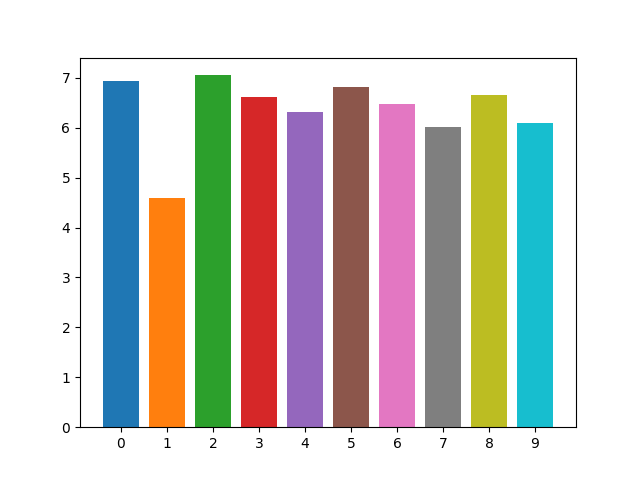
\includegraphics[width=0.49\linewidth]{convolutional_VAE_new_idea_KL_4e-2_10k_epochs_3D_errors}
\end{center}
\caption{The figure illustrates the test errors of the variational autoencoder with the posterior chosen customly with bottleneck $n_b=3$ and KL-coefficient $\l = \num{4e-2}$, where each bar represents the averaged test errors over the entire MNIST dataset for each of the ten digits.}\label{fig:convolutional_VAE_new_idea_KL_4e-2_10k_epochs_3D_errors}
\end{figure}


We realise that we managed to successfully train a variational autoencoder with a comparatively low KL-coefficient of $\l=\num{4e-2}$, where in contrast, the common approach failed, see Figure \ref{fig:convolutional_VAE_snd_KL_4e-2_10k_epochs_3D_inference} or Figure \ref{fig:convolutional_VAE_snd_KL_4e-2_10k_epochs_3D_errors}. Moreover, our network even outperfoms the discriminative model (with the same bottleneck), see e.g. Figure \ref{fig:linear_AE_3d_amsgrad_inference}. Now, we want to take a look at the reconstruction capability for this approach with bottleneck $n_b=10$, see Figure \ref{fig:convolutional_VAE_new_idea_KL_4e-2_10k_epochs_10D_inference} with the corresponding reconstruction errors, see Figure \ref{fig:convolutional_VAE_new_idea_KL_4e-2_10k_epochs_10D_errors}.

\begin{figure}
\begin{center}
      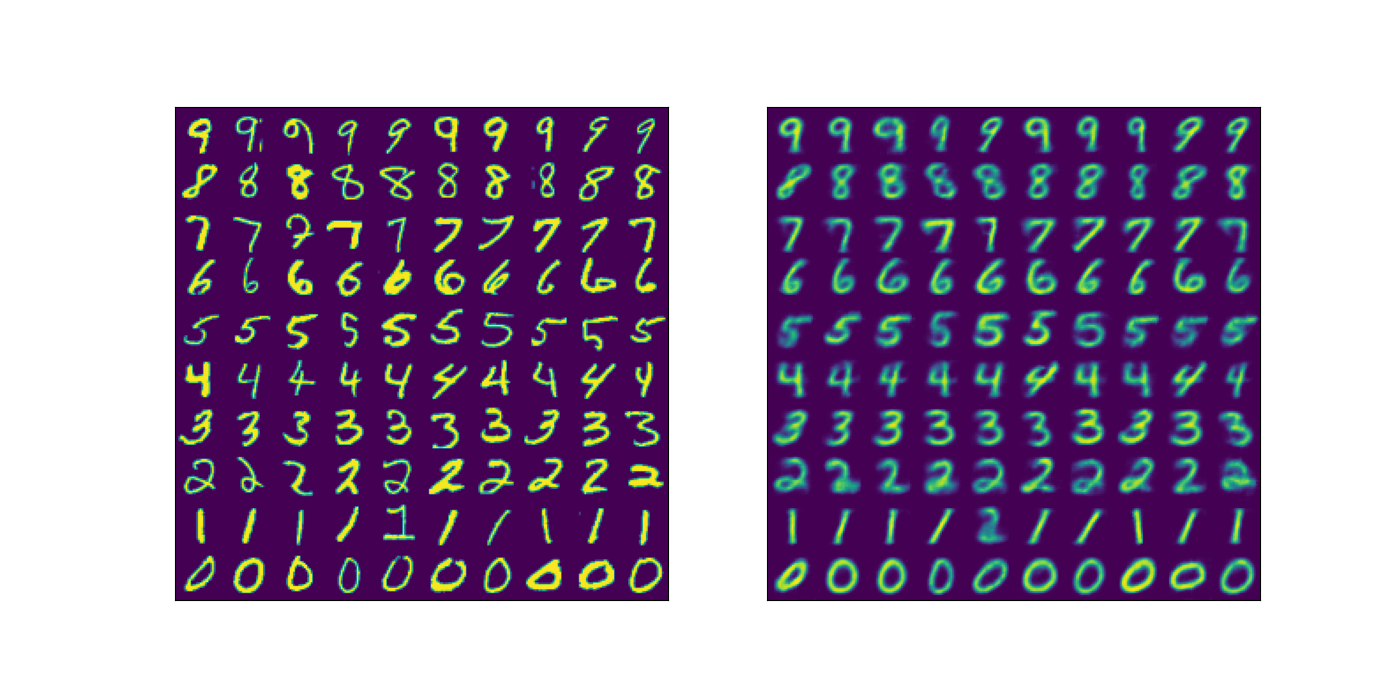
\includegraphics[trim = 15mm 10mm 15mm 15mm, clip, width=\linewidth]{convolutional_VAE_new_idea_KL_4e-2_10k_epochs_10D_inference}
\end{center}
\caption{On the left-hand side, the figure illustrates $100$ original digits from the MNIST dataset. On the right-hand side, the figure illustrates the same digits after feeding them through the variational autoencoder with the posterior chosen customly with bottleneck $n_b=10$ and KL-coefficient $\l=\num{4e-2}$ to produce a reconstruction.}\label{fig:convolutional_VAE_new_idea_KL_4e-2_10k_epochs_10D_inference}
\end{figure}


\begin{figure}
\begin{center}
      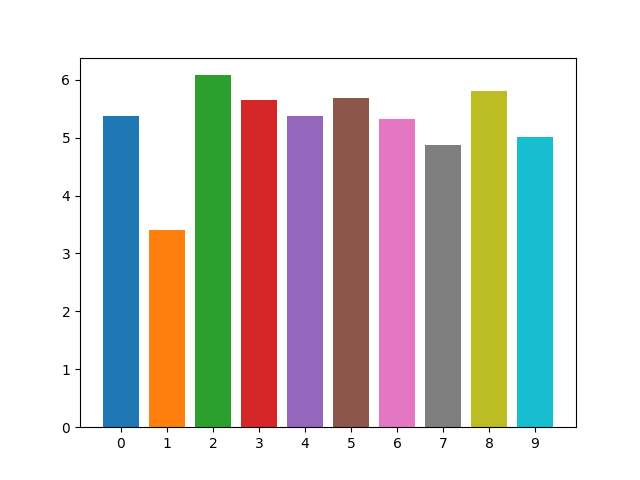
\includegraphics[width=0.49\linewidth]{convolutional_VAE_new_idea_KL_4e-2_10k_epochs_10D_errors}
\end{center}
\caption{The figure illustrates the test errors of the variational autoencoder with the posterior chosen customly with bottleneck $n_b=10$ and KL-coefficient $\l = \num{4e-2}$, where each bar represents the averaged test errors over the entire MNIST dataset for each of the ten digits.}\label{fig:convolutional_VAE_new_idea_KL_4e-2_10k_epochs_10D_errors}
\end{figure}


Increasing the bottleneck one last time to $n_b=64$ gives us the reconstructions in Figure \ref{fig:convolutional_VAE_new_idea_KL_4e-2_10k_epochs_64D_inference} and reconstruction errors in Figure \ref{fig:convolutional_VAE_new_idea_KL_4e-2_10k_epochs_64D_errors}. We see that the reconstructions are comparable to the common approach of choosing the standard normal density as the density the KL-divergence refers to. This is clearly visible if one compared the reconstruction errors, see Figure \ref{fig:convolutional_VAE_new_idea_KL_4e-2_10k_epochs_64D_errors} and \ref{fig:convolutional_VAE_snd_KL_4e-2_10k_epochs_64D_errors}.


\begin{figure}
\begin{center}
      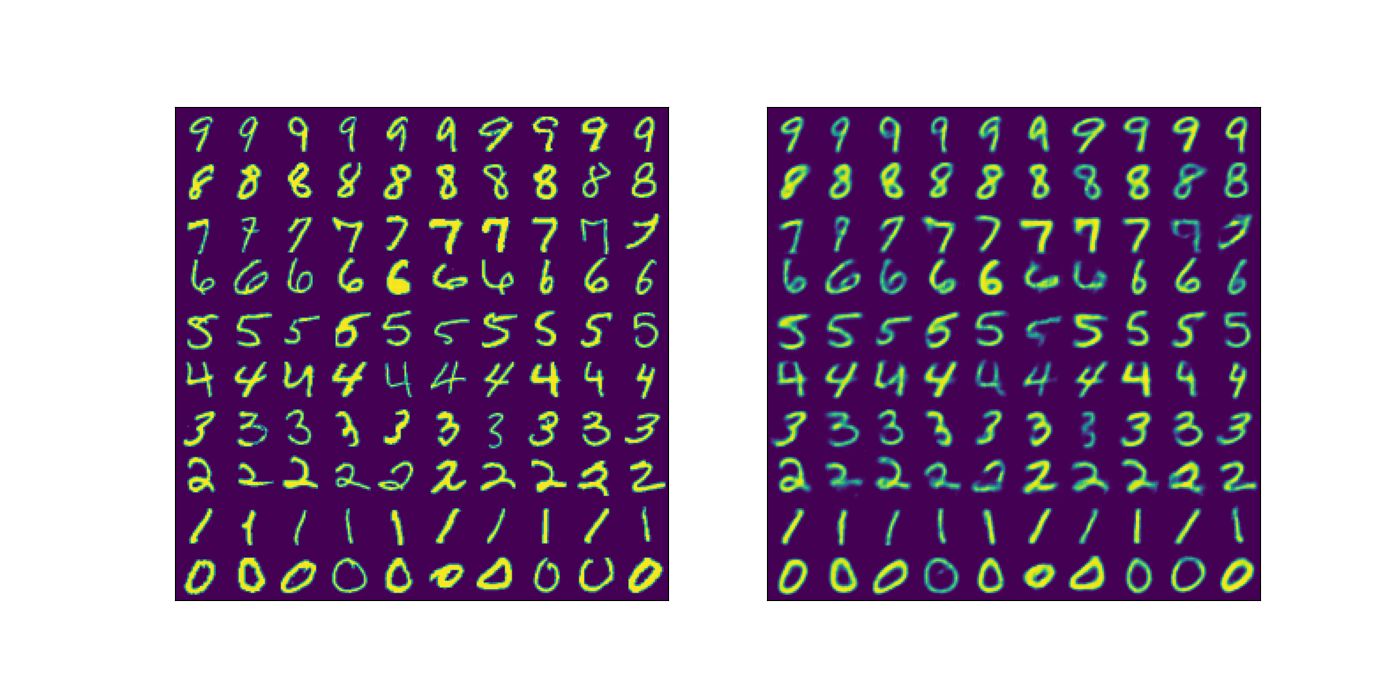
\includegraphics[trim = 15mm 10mm 15mm 15mm, clip, width=\linewidth]{convolutional_VAE_new_idea_KL_4e-2_10k_epochs_64D_inference}
\end{center}
\caption{On the left-hand side, the figure illustrates $100$ original digits from the MNIST dataset. On the right-hand side, the figure illustrates the same digits after feeding them through the variational autoencoder with the posterior chosen customly with bottleneck $n_b=64$ and KL-coefficient $\l=\num{4e-2}$ to produce a reconstruction.}\label{fig:convolutional_VAE_new_idea_KL_4e-2_10k_epochs_64D_inference}
\end{figure}


\begin{figure}
\begin{center}
      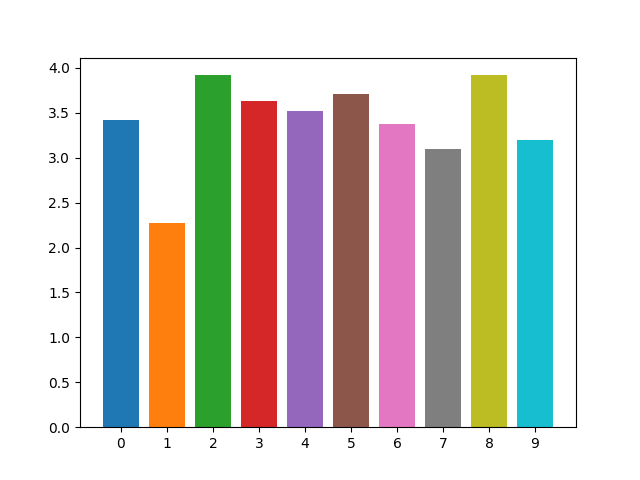
\includegraphics[width=0.49\linewidth]{convolutional_VAE_new_idea_KL_4e-2_10k_epochs_64D_errors}
\end{center}
\caption{The figure illustrates the test errors of the variational autoencoder with the posterior chosen customly with bottleneck $n_b=64$ and KL-coefficient $\l = \num{4e-2}$, where each bar represents the averaged test errors over the entire MNIST dataset for each of the ten digits.}\label{fig:convolutional_VAE_new_idea_KL_4e-2_10k_epochs_64D_errors}
\end{figure}

Lastly, we want to analyse how the variational autoencoder behaves if we try to generate new samples. To do so, we add some $\e\sim \mathcal{N}(0,1)$ noise to the mean of the encoded probability density and then feed a sample through the decoding part of the neural network. This way we generate ten images for each of the ten digits. The generated samples are visualised in Figure \ref{fig:convolutional_VAE_better_generations_new_idea}.


\begin{figure}
\begin{center}
   \begin{minipage}[b]{0.60\linewidth}
      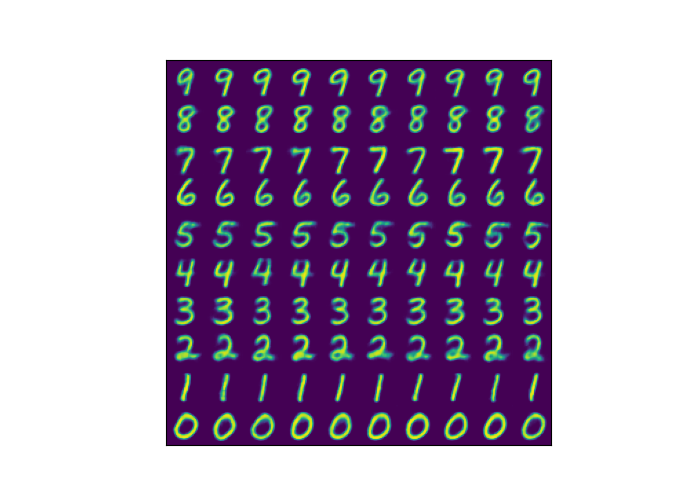
\includegraphics[trim = 15mm 10mm 15mm 10mm, clip, width=\linewidth]{convolutional_VAE_new_idea_KL_4e-2_10k_epochs_64D_generated_optimal}
	\end{minipage}
\end{center}
\caption{The figure illustrates $100$ generated samples by the variational autoencoder with bottleneck $n_b=64$ and customly chosen posterior. Where we applied some noise to the mean of the encoded densities.}\label{fig:convolutional_VAE_better_generations_new_idea}
\end{figure}

As we can clearly see, the generated samples look much better than with the common approach in literature, see Figure \ref{fig:convolutional_VAE_better_generations}. Furthermore, since we chose the mean of the encoded distribution in advance, we do not have to determine it by computing the average of the encoded means, which is quite expensive since one has to consider many samples in order to compute an accurate average. Therefore, we can simply take mean chosen a priori and apply some noise to it.
